\chapter{Datapath and Control}
The datapath and control design methodology break the design
of digital systems into two components: a datapath and a control 
unit.  The datapath is responsible for all the data manipulations
and the control unit is responsible for sequencing the
actions of the datapath.  The datapath is constructed from the basic 
building blocks presented in Chapters 4 and 6.  The control unit is
a FSM.  

A digital system built using the datapath and control design approach
is still a digital system whose inputs and outputs can be categorized
using the terminology introduced Figure~\ref{fig:Asys}.  The 
digital system shown in this figure is broken down into two components,
a datapath and a control unit.  The addition of a clock and a reset signal for the 
sequential logic elements yields Figure~\ref{fig:Abstract}.

\begin{figure}[ht]
\center{\scalebox{0.7}{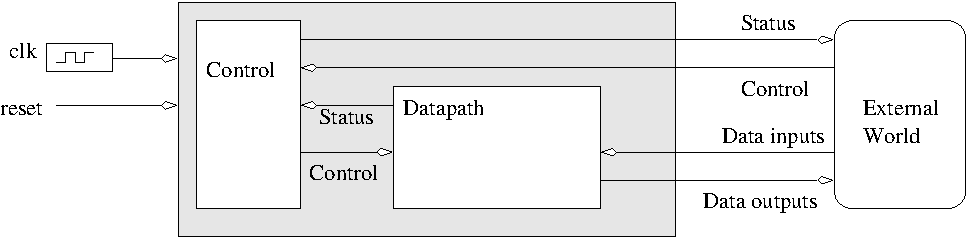
\includegraphics{./Fig8/Abstract}}}
\caption{An abstract digital system constructed from a datapath and
a control unit.}
\label{fig:Abstract}
\end{figure}
\label{page:Abstract}

The datapath can perform a variety of data transformations.  The control 
unit instructs the datapath which transformation to perform using a set 
of control signals called the control word.  An often overlooked portion 
of the control word are signals provided by the external world such as
the acknowledge signal in a two-line handshake.  The datapath 
provides status information about the state of its transformation to the 
control unit.  Then, the control unit uses this information to determine 
the next instruction to the datapath.

A structured approach to designing digital systems with a
datapath and control architecture is offered next.

%% ----------------------------------Conversion-----------------------
\section{Conversion}
Building digital systems using the datapath and control approach is a
three-step process.

\begin{enumerate}
\item Write an algorithmic description for the solution to the problem.
\item Parse the algorithmic description into datapath building blocks and control states.
\item Define the MIEs and OEs for the control unit.
\end{enumerate}

The algorithmic descriptions are written in a simple programming language.
The algorithmic description is then transformed into hardware by
parsing the algorithm one line at a time.  Each statement in the 
algorithm introduces additional building blocks in the datapath and
additional states in the control unit.  After the algorithm is finished
being parsed, the design is completed by deriving the MIEs and OEs of the 
FSM.

\subsection{Word Statement to Algorithm}
The programming language used to formalize an algorithmic
solution to design problem is a derivative of the popular C-programming
language referred to as mini-C.  The mini-C programming language contains
four types of statements.

\begin{itemize}
\item \verb^if (condition) then BODY_1 else BODY_2^
\item \verb^for (i=A; i<B; i+= 1) BODY^
\item \verb^while(condition) BODY^
\item \verb^X = value^
\end{itemize}

The term ``BODY" is a place holder for 0 or more statements.  In this way, 
statements can be nested.  For example, the body of a for loop may contain
a for loop, the body of which may contain a while loop, etc...  In addition
to statements, the mini-C language also requires variables to hold the state
of the program.

In digital circuit design, the variable types in the mini-C language 
are limited to be either binary or 2's-complement integers.  Arrays 
of these types are common.  Limiting the discussion to integer types  
is not an inherent limitation of the mini-C language, rather it limits
the discussion to the essential points of the design process.  Complex
types like floating-point numbers can be accommodated if the necessary
representations and hardware are developed.

No effort is made to explain the process of transforming a word statement
into an algorithm; the process should be a familiar task from writing 
programs.  Rather, consideration of the transformation
of the algorithm into hardware is presented.

%%--------------------------------ALGORITHM TO CIRCUIT---------------------
\subsection{Algorithm to Circuit}
From an algorithmic statement, its conversion into hardware is desired.
The conversion  is accomplished by parsing the algorithm.  In 
computer science, parsing is the process of analyzing a program for its 
structure.  Here, parsing means analyzing
a program line-by-line, sequentially, from the first line to the last line, to 
determine its hardware structure.  The analysis process takes a line 
of code, a mini-C statement, and transforms it into some additional
building blocks in the datapath and some additional states in
the control unit.  When the parsing is complete, the datapath 
has all the functionality present in the algorithm, and the control
unit has all the control structures present in the algorithm.

As an example of the process, a familiar statement first introduced
in Chapter 4, the if/then/else statement, is transformed.

\begin{description}
\item[]\verb^if (condition) then BODY_1 else BODY_2^

When an if/then/else statement is encountered in a program, 
\verb^BODY_1^ is executed when the condition is true.  If condition 
is false, then \verb^BODY_2^ is executed.  \verb^BODY_1^ and \verb^BODY_2^ 
contain 0 or more statements.  Typically, the datapath computes 
the condition using a comparator.  In such a case, the datapath 
requires a comparator, the output of which is
the status signal shown in Figure~\ref{fig:IfThen}.  

While the control unit is in state {\bf IfThen}, the condition 
is being evaluated, the status signal
is being communicated to the control unit, and the control
unit is deciding whether to transition to either the 
{\bf BODY}$_1$ or {\bf BODY}$_2$ states.  When the clock 
edge arrives, the control unit will transition to its next state.
The {\bf BODY}$_1$ or {\bf BODY}$_2$ states contain the entire 
collection of states derived by parsing all the statements in 
their respective bodies.  Regardless of which path the control 
unit takes, both threads return to the {\bf Next} state, which 
is the next statement after the if/then/else statement in the algorithm.

\begin{figure}[ht]
\center{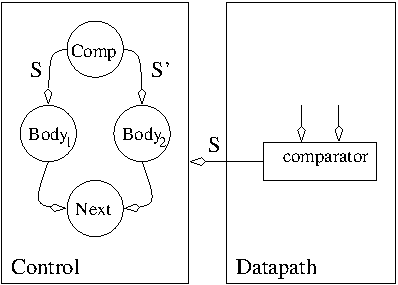
\includegraphics{./Fig8/IfThen}}
\caption{The datapath and control components required to realize
an if/then/else structure.}
\label{fig:IfThen}
\end{figure}

\item[]\verb^for(i=A; i<B; i+=1) BODY^

When a for loop is encountered in a program, \verb^BODY^ is 
executed B-A times and the value of \verb^i^ is available 
for use inside \verb^BODY^.  \verb^BODY^ contains 
zero or more statements.  A for statement requires a counter and a 
comparator arranged as shown in Figure~\ref{fig:For}.  The initial
value of the for loop is the data input to the counter.  The 
output of the counter is the \verb+i+ variable of the for loop.  The
\verb+i+ variable is compared to the terminal value of the for loop.
The status of this comparison is passed to the control 
unit so that the control unit knows to terminate the for loop
when the counter has reached its terminal value.

The control unit sequences the actions of the hardware in the
datapath.  The execution of the for loop begins with an 
initialization of the counter in the {\bf Init} state.  In this state,
the control unit asserts a load signal on the control lines to
the counter causing the counter to be initialized to A.  On the
next clock edge, the counter loads A and the control unit
transitions to the {\bf Comp} state.  In this state, the control unit
does nothing, giving the comparator time to determine the 
relative magnitude of i and B, and to assert its L output
to the control unit in the form of a status signal. The control
unit uses the status signal to either execute the body of 
the for loop, or to exit the for loop and proceed with
the next instruction after the for loop.  The {\bf Body} state 
represents the collection of states derived by parsing all 
the statements in the body of the for loop.  At the end of the 
for loop's body, the control unit enters the {\bf Inc} state where the 
control unit asserts an increment signal on the control lines 
to the counter.  This assertion causes the counter to count up on the 
next edge which also causes the control unit to transition
back to the {\bf Comp} state.

\begin{figure}[ht]
\center{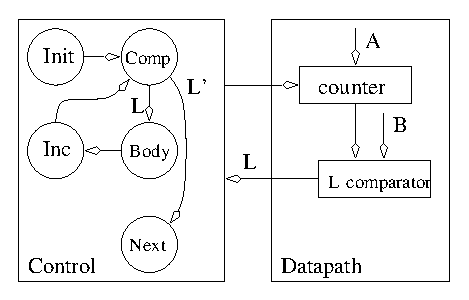
\includegraphics{./Fig8/For}}
\caption{The datapath and control components required to realize
a for loop.}
\label{fig:For}
\end{figure}

\item[]\verb+while(condition) BODY+


When a while loop is encountered in a program, \verb^Body^ is executed 
while the condition is true.  Typically, 
the datapath computes the condition using a comparator, the 
output of which is the status signal shown in 
Figure~\ref{fig:While}.  While the control unit is in state
{\bf Comp}, the condition is being evaluated, the status signal is
being communicated to the control unit, and the control unit 
deciding on whether to transition to either the {\bf Body} or 
{\bf Next} states.  The {\bf Body} state represents the 
collection of states derived by parsing all the statements 
in the body of the while loop.

In some cases the status signal may be determined by some external 
source.  Then, the status line shown in Figure~\ref{fig:While} 
as emanating from the datapath would in fact be sent in from the 
external world as shown in Figure~\ref{fig:Abstract}.

\begin{figure}[ht]
\center{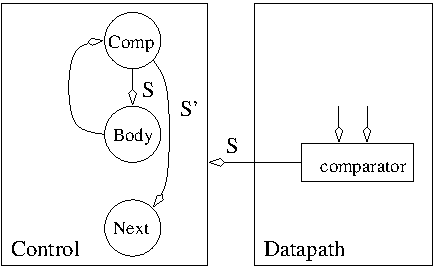
\includegraphics{./Fig8/While}}
\caption{The datapath and control components required to realize
a {\bf while} statement.}
\label{fig:While}
\end{figure}

\item[]\verb^X = value^

When an assignment statement is encountered in a program, 
\verb^X^ is assigned a new value.  This statement is realized by 
placing a register in the datapath whose input is the 
value on the right-hand side of the assignment statement.  
In order to make the assignment, the control unit
enters the {\bf Op} state, where it asserts a load signal on the
registers control input.  On the next positive edge of the 
clock, the register loads its value and the control unit
moves on to the {\bf Next} state.

The size of the register storing X is determined by the range
of values  required to be stored in X.  In some
cases, this size is defined by the word statement; in 
other cases, the designer must make a judgment call on a reasonable
value range.

Statements like \verb^X = X+Y^ often occur in 
algorithms.  In cases when a variable appears on both the left-hand
and right-hand side of an assignment statement, feedback must
be employed as shown in Figure~\ref{fig:Op}.  In this case, the 
output from the X register is added to Y, the output of the summation
is sent to the data input of the X register.  The control unit
asserts a load signal on the X register's control input when
it is in the {\bf Op} state.  Most likely, the control unit would assert
a hold signal on the Y register's control input while it
was in the {\bf Op} state.

\begin{figure}[ht]
\center{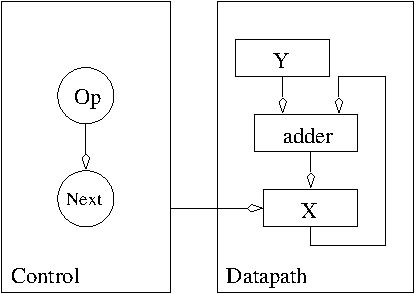
\includegraphics{./Fig8/Op}}
\caption{The datapath and control components required to realize
an assignment statement of the form X+Y.}
\label{fig:Op}
\end{figure}

What prevents the X register from rapidly adding Y to itself 
multiple times?  The answer is that the X register will 
only latch X+Y on the positive edge of the clock.  So 
X+Y cannot ``get into" the X register until the positive 
clock edge.

A variable often appears on the left-hand side (LHS) 
of two or more assignment statements.  For example, consider a
algorithmic description which contains the statements \verb+X=Y+ 
and \verb+X=Z+.  In this case, the variable \verb^X^ appears on the LHS
of two assignments.  Since the variable \verb^X^ is stored in a register
which has a single input, a problem occurs because there are two 
different sources for the input.  This conflict is resolved by
inserting a mux between the two data sources and the single
data input of the X register as shown in Figure~\ref{fig:2Source}.
The control unit aids in resolving this conflict by asserting 
control$_1$ to route the correct value to the data input of 
register X when the control unit asserts a load signal on the 
control$_2$ line.

\begin{figure}[ht]
\center{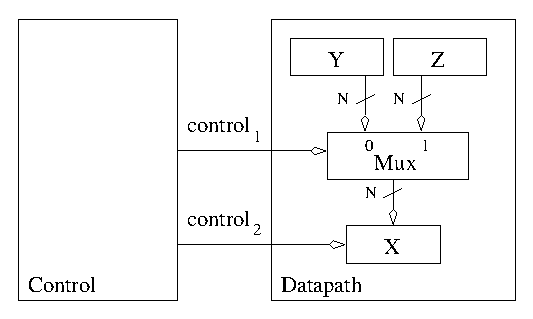
\includegraphics{./Fig8/2Source}}
\caption{The datapath and control components required to resolve
the problem of a register requiring two different sources of
data input.}
\label{fig:2Source}
\end{figure}

\end{description}

%%-----------------------HERE------------------------------

\subsection{Control Word}
After the algorithm is parsed, the design of the datapath is complete
and the architecture of the control unit is complete.  The details of 
the control unit, its MIEs and OEs, remain to be defined.  A 
one-hot encoding of the states means the MIEs can be derived directly
from the state diagram constituting the control unit.  The real work
comes from the definition of the control word for each state.

\begin{quote}
A control word is a complete listing of the names and meanings of 
all the control signals sent {\bf from} the control unit {\bf to} the
datapath.  
\end{quote}

Chapters 4 and 6 introduced a variety of basic building
blocks with a variety of inputs and outputs.  Table~\ref{table:bbblist}
summarizes all inputs and outputs from these basic building blocks
as well as their page numbers.

\begin{table}
{\small
\begin{tabular}{|l|l|l|l|l|l|} \hline
Device      & Page & Data in     & Data out & Status   & Control \\ \hline
N:M Decoder & \pageref{page:dec}          & 1 bit       & M bits  & 	& N bits  \\ \hline
N:1 Mux     & \pageref{page:mux}          & N bits  & 1 bit    & 	&  $\log_2(N)$ bits  \\ \hline
M-bit N:1 Mux   & \pageref{page:wmu}          & N, each M-bits  & M bits & 	&  $\log_2(N)$ bits  \\ \hline
N-bit adder & \pageref{page:add}          & 2, each N-bits & N bits & Overflow &   \\ \hline
N-bit add/sub & \pageref{page:as}         & 2, each N-bits & N bits & Overflow & 1 bit  \\ \hline
N-bit comparator & \pageref{page:com}     & 2, each N-bits &  & 3 bits &   \\ \hline
BCD to 7-segment & \pageref{page:7seg}  & 4 bits & 7 bits & &   \\ \hline
N-bit priority encoder & \pageref{page:prior}  & N bits & $\log(N)$-bits & &   \\ \hline
N-bit register & \pageref{page:reg}       & N bits & N-bits &  & 1 bit  \\ \hline
N-bit shift register & \pageref{page:shi} & N bits & N-bits &  & 2 bits  \\ \hline
N-bit counter & \pageref{page:counter}        & N bits & N bits &  & 2 bits  \\ \hline
Three state buffer& \pageref{page:tsb}      & N bits & N bits & & 1 bit  \\ \hline
N:M RAM & \pageref{page:ram}              & $\log_2(N)$ bits, M bits & M bit & & 2 bits  \\ \hline
N-bit Bus transceiver & \pageref{page:bus}      & N bits & N bits & & 2 bit  \\ \hline
\end{tabular}
}
\caption{The list of all the basic building blocks and some of their attributes.}
\label{table:bbblist}
\end{table}
\label{page:boxlist}

The control word is defined by listing the control inputs and their effects
for every basic building block in the datapath.  The control word defines 
the language of the datapath; any task performed by the datapath must
be expressed using this collection of bits.  The list of control inputs
forms the header of the control word table, the table which 
contains the control word for every state.  The rows of the control word 
table are labeled with all the state names used in the control unit.  Then,
the actions each state needs to perform in the datapath are translated 
into the language defined by the control word.  

In order to give this discussion concrete meaning, a circuit from Chapter
6, the minimum search problem, is reexamined.

%% ----------------Minimum Search -----------------------

\section{Minimum Search}

The minimum search problem on page~\pageref{page:minsearch} is reexamined 
for two reasons.  First, the solution presented was unable to initialize
the min register.  Second, the problem will now be solved using the 
datapath and control approach, allowing the comparison of two different 
control approaches.  All control
decisions in a datapath and control circuit are centralized in 
the control unit, whereas the control strategy used in the Chapter 
6 solution was distributed throughout the circuit.

\begin{quote}
Design a digital circuit that looks for the smallest 8-bit integer 
in a 128x8 RAM.  The numbers are stored at addresses 
$0\ldots 99$. Assume the RAM is preloaded with data.
\end{quote}

The strategy used to solve this problem is the same as the strategy
outlined on page~\pageref{page:minsearch}: Compare successive elements
of the RAM to the smallest value found so far, and update the smallest value
if the RAM value is smaller.  The caveat of the strategy is to 
initialize the value of the register holding
the minimum value found so far to the largest
possible 8-bit value, 0xFF.

\begin{verbatim}
1.  min = 0xFF;               // Set the min reg to largest 8-bit value
2.  for (i=0; i<100; i++) {   // Search through the entire array
3.      MBR=RAM[i];           // Read an 8-bit value from the RAM
4.      if (MBR<min) then     // If MBR is smaller than min
5.          min = MBR;        //   then set min to the smallest value
6.  } // end for
\end{verbatim}

Now the translation of this algorithm to hardware proceeds by examining
line-by-line the algorithm and transforming each statement into some datapath
and control.

{\bf Line 1.} The min register is initialized to the largest 8-bit integer,
in this case hexadecimal FF.  When this assignment statement is parsed
according to Figure~\ref{fig:Op}, one state is added to
the control unit and a register to the datapath.  The state is called
{\bf InitMin}. Other initialization states in the 
control unit are to be expected and each should be given a distinct name.  An 8-bit 
register, labeled min, is placed in the datapath.  Since min is on the 
LHS of two assignment statements (Line 1 and Line 5), place a 8-bit 2:1 
mux in front of the min register; see Figure~\ref{fig:2Source}.  When
the control unit is in the {\bf InitMin} state, it asserts a load
signal on the min register's control input and should route 0xFF through
the min register's mux.

{\bf Line 2.} The for loop is used to search every address in the 
RAM looking for the smallest value.  When this for loop is parsed 
according to Figure~\ref{fig:For}, three states are added to
the control unit and a counter and comparator is added to the datapath. In 
Figure~\ref{fig:MinSearch}, the {\bf InitI, CompC, Inc} states correspond 
to the {\bf Init, Comp, Inc} in Figure~\ref{fig:For}, respectively. The 
body of the for loop is composed of Lines 3-5.  The {\bf Body} state of 
the for loop in Figure~\ref{fig:For} is composed of the 
{\bf Read, CompM, NewMin} states in Figure~\ref{fig:MinSearch}.  The
output of the counter is sent to a comparator whose output, labeled
IC, is sent to the control unit so, allowing the for loop to acknowledge when
completed. 

When the control unit is in the {\bf InitI} state, it asserts a load
signal on the counter's control input.  In the {\bf CompC} state, the control unit
should have the counter hold its value.  In the {\bf Inc} state, the control
unit should assert an increment signal on the counter's control input.

{\bf Line 3.} In this line, the RAM is read and its value is stored in the MBR.  When this
assignment statement is parsed according to Figure~\ref{fig:Op}, one state is added 
to the control unit, and a register and RAM is added to the 
datapath. The state {\bf Read} in Figure~\ref{fig:MinSearch} corresponds to the state
{\bf OP} in Figure~\ref{fig:Op}.  Since the expression \verb+RAM[i]+ is on the RHS
of the assignment statement, the RAM provides the data to the 
MBR register.  When the control unit is in the {\bf Read} state, 
a read signal is asserted on the RAM's control input and a load signal is asserted 
on the MBR register's control input.

{\bf Line 4.}  The output of MBR is compared to min.  When the if/then/else statement
is parsed according to Figure~\ref{fig:IfThen}, one state is added
to the control unit and a comparator is added to the datapath.  The state {\bf CompM} in 
Figure~\ref{fig:MinSearch} plays the role of the state {\bf IfThen} in Figure~\ref{fig:IfThen}.
This state uses the output of the comparator labeled MC to determine which 
state to enter next.  If min is less than the MBR, MC=1 and the 
control unit 
goes to the state {\bf NewMin} in the next clock cycle.  Otherwise, the control goes 
to the state {\bf Inc}.

{\bf Line 5.}  The line of code is only executed if MBR is less than min.  
When the assignment statement is parsed according to Figure~\ref{fig:Op},
one state is added to the control unit and no additional hardware
to the datapath because the min and MBR registers are already in the datapath.
The state {\bf NewMin} in Figure~\ref{fig:MinSearch} corresponds to the state
{\bf OP} in Figure~\ref{fig:Op}.  When the control unit is in the {\bf NewMin}
state, a load signal is asserted on the min registers control input 
and routes MBR through the min register's mux.

{\bf Line 6.}  The line of code halts the machine.  When the while loop is parsed,
one state is added to the control unit and no hardware to the 
datapath.  The {\bf Done} state in Figure~\ref{fig:MinSearch} corresponds to 
the state {\bf Comp} in Figure~\ref{fig:While}.  The unconditional self arc
to/from the {\bf Done} state halts a FSM when it gets to the {\bf Done}
state.  However, in most cases the circuit will restart its primary 
operation from the beginning when it has completed one iteration. 

\begin{figure}[ht]
\center{\scalebox{0.7}{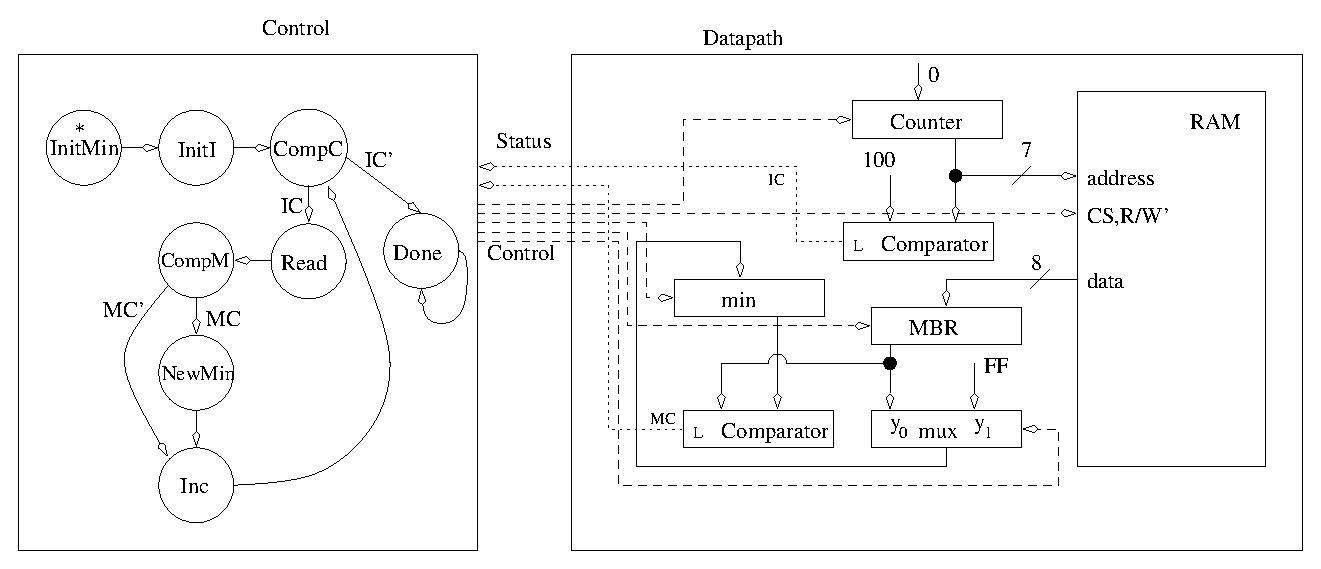
\includegraphics{./Fig8/MinSearch}}}
\caption{The datapath and control components required to implement
the minimum search circuit.}
\label{fig:MinSearch}
\end{figure}

The dotted lines representing the status information are generated in the 
datapath by comparators and sent to the control unit which uses them to 
decide which course of action to take next.  The dashed lines 
represent control information generated by the control unit to instruct
the datapath which actions to perform.  The control lines should not be 
drawn on the datapath and control circuits as they unnecessarily clutter 
the figure and do not add any useful information.  Since the basic 
building blocks are assumed to be controlled by the control unit, 
assume these connections are present even when they are not drawn.
Since the control unit handles all processing of the status bits,
the status outputs from all the comparators in the datapath must
be sent to the datapath.  Since it is implicit that the status bits
are sent to the control unit, they do not need to be drawn all the
way to the control unit.  Draw just enough of the status output 
in order to fit the name of the status signal.  

Since a one-hot encoding of the states is employed, MIEs are determined 
for the control unit by inspection as shown below.

$\begin{array}{l}
D_{IM} = 0 \\
D_{II} = Q_{IM} \\
D_{CC} = Q_{II} + Q_{I} \\
D_{R}  = Q_{CC} * IC \\
D_{CM} = Q_{R}  \\
D_{D}  = Q_{CC} * IC' \\
D_{NM} = Q_{CM} * MC \\
D_{I}  = Q_{NM} + Q_{CM}*MC' \\
\end{array}$

The control word for the circuit is determined by listing every control
input in the datapath along with its associated action.  In 
Figure~\ref{fig:MinSearch}, the collection of dashed lines forms the 
control word.  It is a good idea to form the control word while parsing 
the algorithm's statements.  By using the table on 
page~\pageref{page:boxlist}, the control input to each 
type of box can be determined.

The header of Table~\ref{table:MinSearch} is the control word table for
the minimum search circuit. Each state is listed as a row in the control 
word table.  The values filled in for each state are determined by examining
the actions each state performs and is discussed next.

\begin{table}
\begin{tabular}{c||c|c|c|c|c|c}  
{\bf State}   & CS       & R/W'   &  Reg Min  & Min mux       & Counter & MBR	\\ \hline
        & 0 off    & 0 write&  0 hold   & 0 load FF     & 00 hold & 0 hold	\\ \hline
        & 1 active & 1 read &  1 load   & 1 load RAM    & 01 load & 1 load	\\ \hline
        &          &        &           &               & 10 count& 		\\ \hline
        &          &        &           &               & 11 reset& \\ \hline \hline
{\bf InitMin } & 0        &    x   & 1         & 0             & 00      & 0   \\ \hline
{\bf InitI }  & 0        &    x   & 0         & x             & 01      & 0   \\ \hline
{\bf CompC }  & 0        &    x   & 0         & x             & 00      & 0   \\ \hline
{\bf Read  }  & 1        &    1   & 0         & x             & 00      & 1   \\ \hline
{\bf CompM }  & 0        &    x   & 0         & x             & 00      & 0   \\ \hline
{\bf NewMin }  & 0        &    x   & 1         & 1             & 01      & 0   \\ \hline
{\bf Inc  }   & 0        &    x   & 0         & x             & 10      & 0   \\ \hline
{\bf Done }   & 0        &    x   & 0         & x             & 00      & 0   \\ 
\end{tabular}
\caption{The control word for the minimum search circuit and its values for each state.}
\label{table:MinSearch}
\end{table}

Determining the values of the control-word bits for each state 
requires understanding what is supposed to happen in each 
state.  For example, parsing Line 1 resulted in adding the 
{\bf NewMin} state.  In this state, the min register was
to be assigned the value 0xFF.  The datapath can accomplish
this by asserting a ``load" to min register and a ``load FF" on the 
Min mux control lines.  All the other basic building blocks 
in the datapath must be inactive, thus the RAM is ``turned off"
and the counter and MBR are told to ``hold" their values.
Closely reading how each line of code is parsed should clearly
indicate which control bits need to be set in the remaining states
of the control unit.

A note about ``don't cares" is appropriate at this point.  As a general
rule, never set the control input of a sequential device to 
``don't care."  The reason is fairly obvious; since sequential devices 
have memory, the effects of a spurious operation will be remembered
and may result in an erroneous operation later on.  On the other hand, a
combinational logic block like an mux can have its control input set 
to ``don't care" when its output is not being used because it will not
remember this decision in the future.  For example, when the min 
register is holding its value, the Min mux's control input is set 
to a ``don't care."  In general,  always set a combinational
logic device's control input to ``don't care" whenever possible to 
communicate the associated device's output is not being used.  While
this will not help reduce the complexity of the control unit when
implemented with a one-hot encoding, it may be helpful under
other encoding schemes.  Once the control word is defined for all the
states, it is time to determine the output equations for the FSM which
is the control unit.

One output equation occurs for each bit in the control word table.
For example, there are eight bits of control in the min search control.
While seven bits of control may seem correct, remember 
the counter requires two bits of control, giving 
eight, total control bits.  The output equation for a control bit is the
OR of the states which cause the output to equal 1.  For example, the 
R/W' output of the control unit equals 1 when the control unit is in the 
{\bf Read} state. Hence, $Z_{RW} = Q_{Read}$.  
All the OEs are summarized in the list below.

$\begin{array}{l}
Z_{CS} = Q_{CM} + Q_{NM} \\
Z_{RW} = Q_{R} \\
Z_{RM} = Q_{IM}  + Q_{NM} \\
Z_{MM} = Q_{NM} \\
Z_{C1} = Q_{I} \\
Z_{C0} = Q_{II} + Q_{NM} \\
Z_{MBR} = Q_{R} 
\end{array}$


In order to understand how the elements of the minimum search circuit 
operate together to complete its task, examine its 
behavior through time using a sequence of modified circuit 
diagrams.  The state diagram representation of 
the control unit is replaced with the circuit diagram 
representation of the one-hot encoded control unit.  When a 
component is active it is shaded.  For example,
when a local signal is asserted on the min register's control
input, the min register is shaded. When a control
or status line is active, it is drawn as a solid line instead 
of a dotted or dashed line.  Each diagram represents the
circuit in one state; the name of the state is written 
underneath the circuit diagram.

The operation of the minimum search circuit starts at time=1
in the {\bf InitMin} state, shown in the upper left of 
Figure~\ref{fig:mintable}.  The flip flop labeled IM ({\bf InitMin}) 
is shaded grey because its output, $Q_{IM}=1$; it is the current state.  
The control word for the {\bf InitMin} state asserts ``load" on the 
min register' control input and ``route FF" to the min mux. Hence, 
these control signals are drawn as solid lines.
The MIE, $D_{II} = Q_{IM}$, means that when the clock edge 
arrives, the control unit transitions to the {\bf InitI} 
state and the min register will latch the value FF.

When the control unit is in the {\bf InitI} state, $Q_{II}=1$
causes the OEs to assert a ``load" on the counter's control
input.  The control unit transitions into state {\bf CompC},
where the IC output of the comparator is used
to send the control unit to the {\bf Read} state.
During this state, the counter is used as the address to
the RAM, which sends its data output to the MBR.  When the 
positive edge of the clock arrives, the MBR latches its
value and the control unit transitions into the {\bf CompM} 
state.  While in this state, the MC output of the comparator
is being used by the control unit to determine whether it 
should transition into the {\bf NewMin} or the {\bf Inc} state
(see Figure~\ref{fig:MinSearch}).  It is assumed that the 
value stored at address 0 in the RAM is less than 0xFF, so
the MC output is 1 and the control unit transitions to the 
{\bf NewMin} state.  In this state, the control 
unit loads the MBR into the min register.  When it is in the {\bf Inc}
state, the control unit is getting ready to enter another loop of the
for loop, by incrementing the counter.  It then transitions
back into the {\bf CompC} state on the next positive clock edge.


\begin{figure}

\begin{tabular}{ll}
\scalebox{0.3}{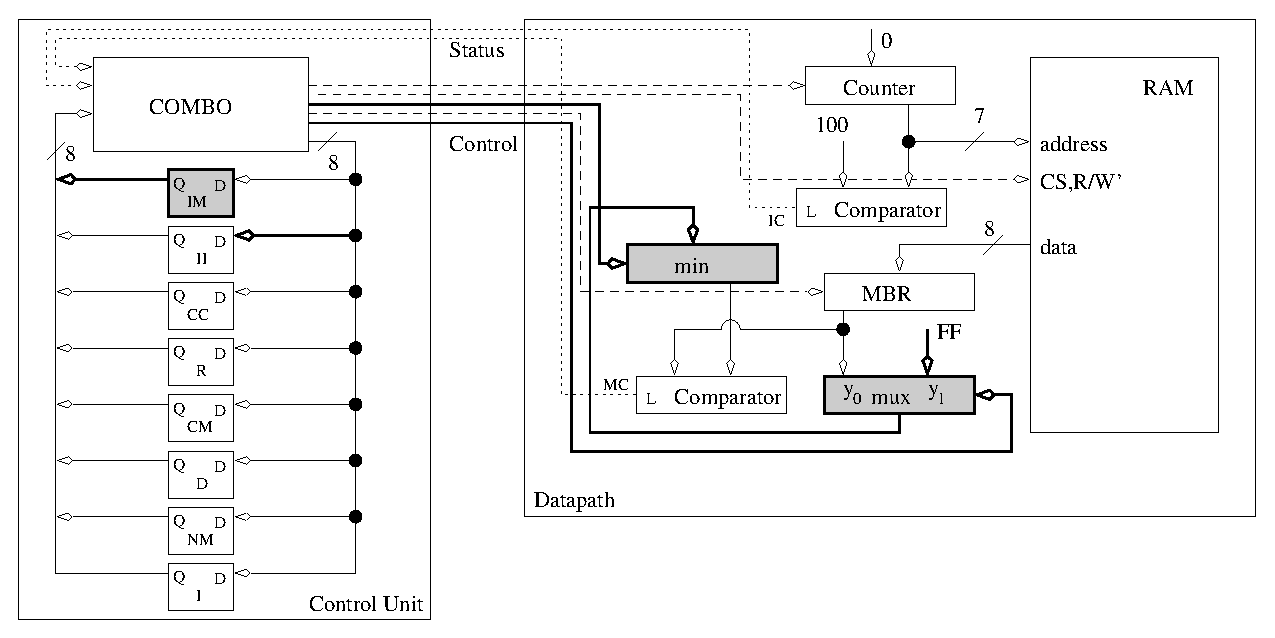
\includegraphics{./Fig8/MinSearch2a}} & 
	\scalebox{0.3}{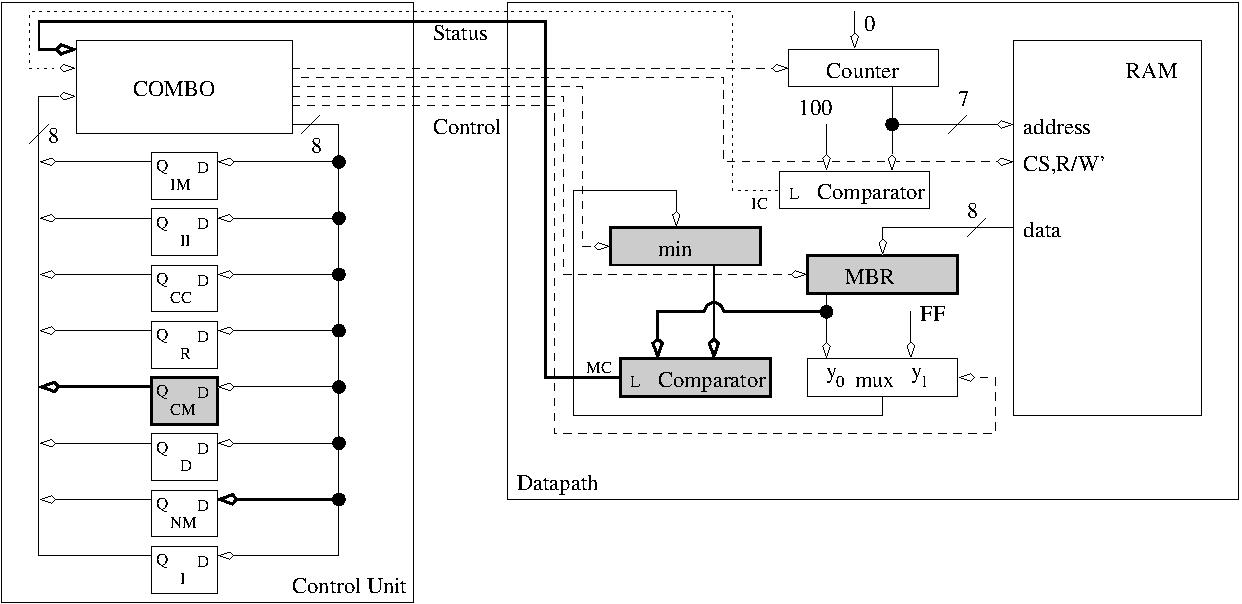
\includegraphics{./Fig8/MinSearch2e}} \\
1. State {\bf InitMin}                               & 5. State {\bf CompM} \\
\scalebox{0.3}{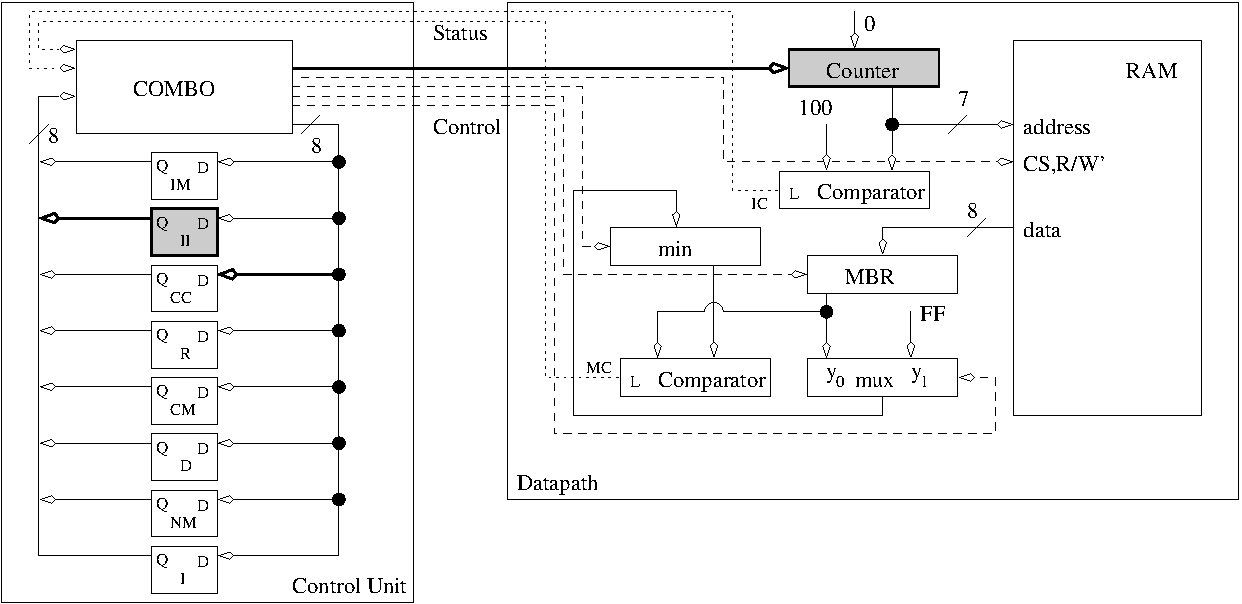
\includegraphics{./Fig8/MinSearch2b}} & 
	\scalebox{0.3}{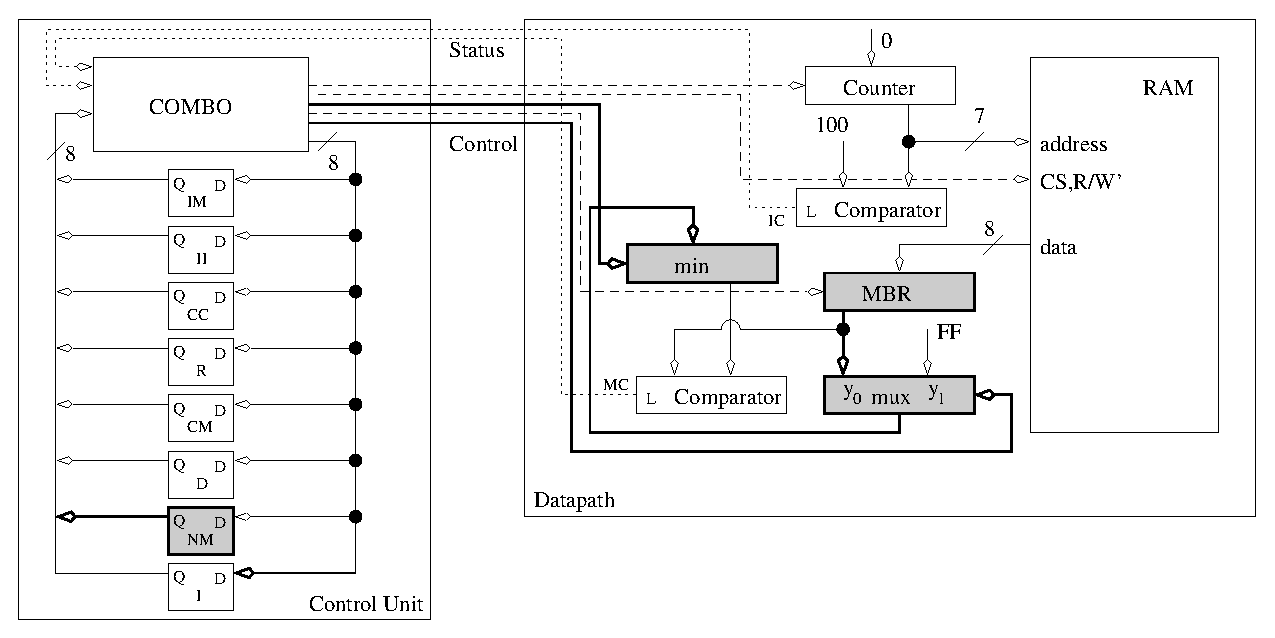
\includegraphics{./Fig8/MinSearch2f}} \\
2. State {\bf InitI}                                 & 6. State {\bf NewMin} \\
\scalebox{0.3}{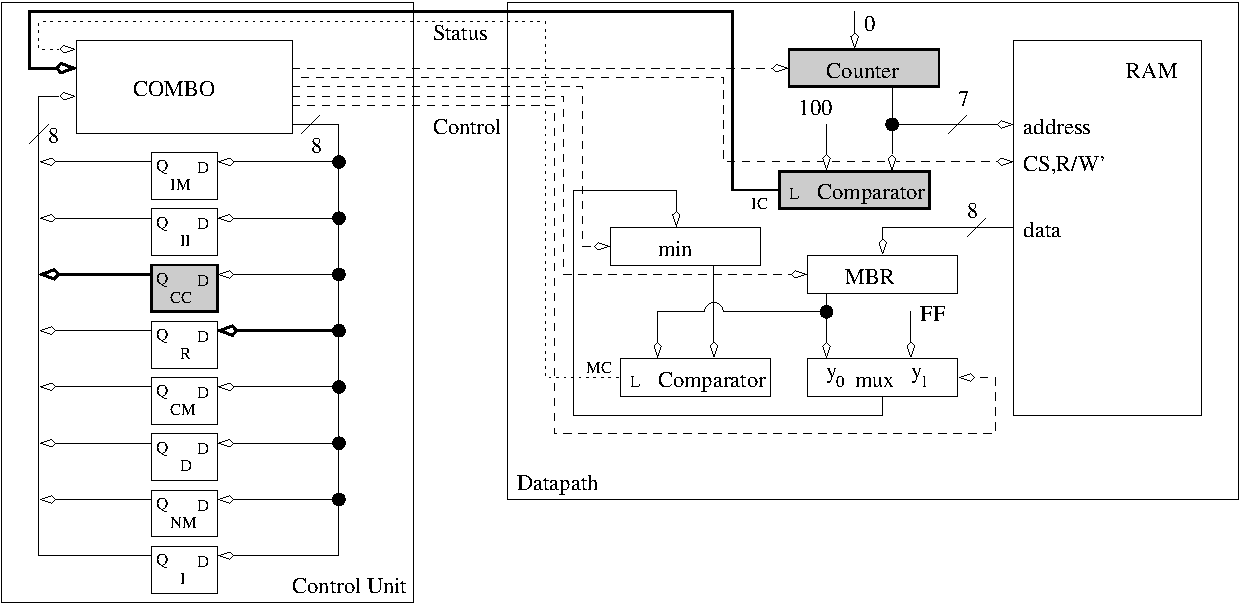
\includegraphics{./Fig8/MinSearch2c}} & 
	\scalebox{0.3}{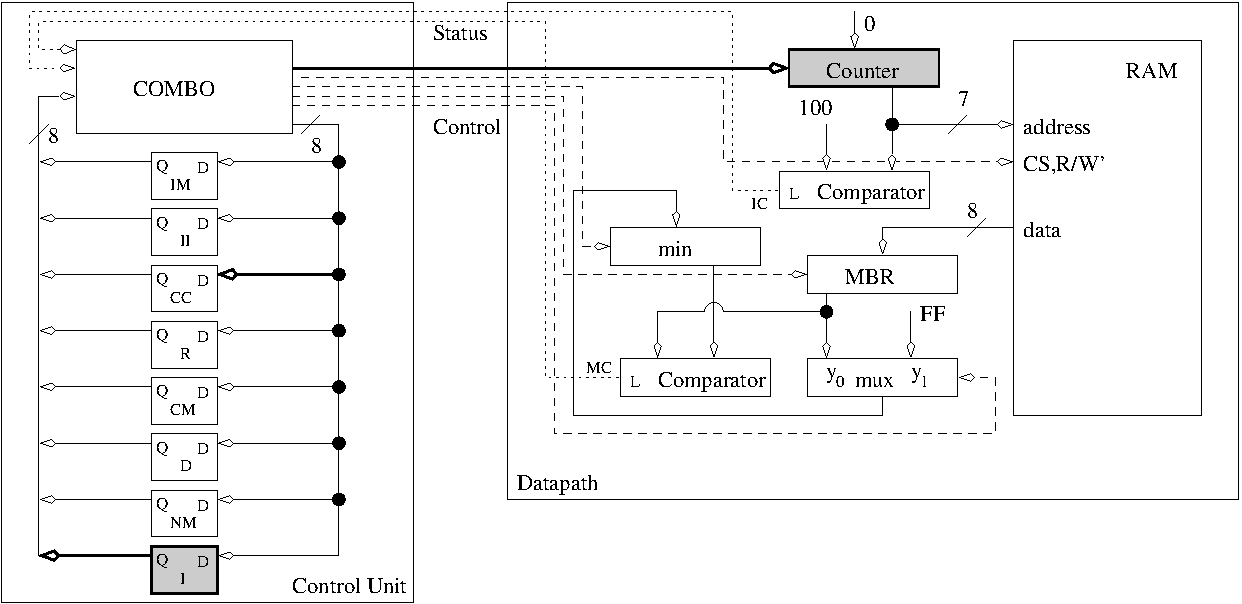
\includegraphics{./Fig8/MinSearch2g}} \\
3. State {\bf CompC}                                 & 7. State {\bf Inc} \\
\scalebox{0.3}{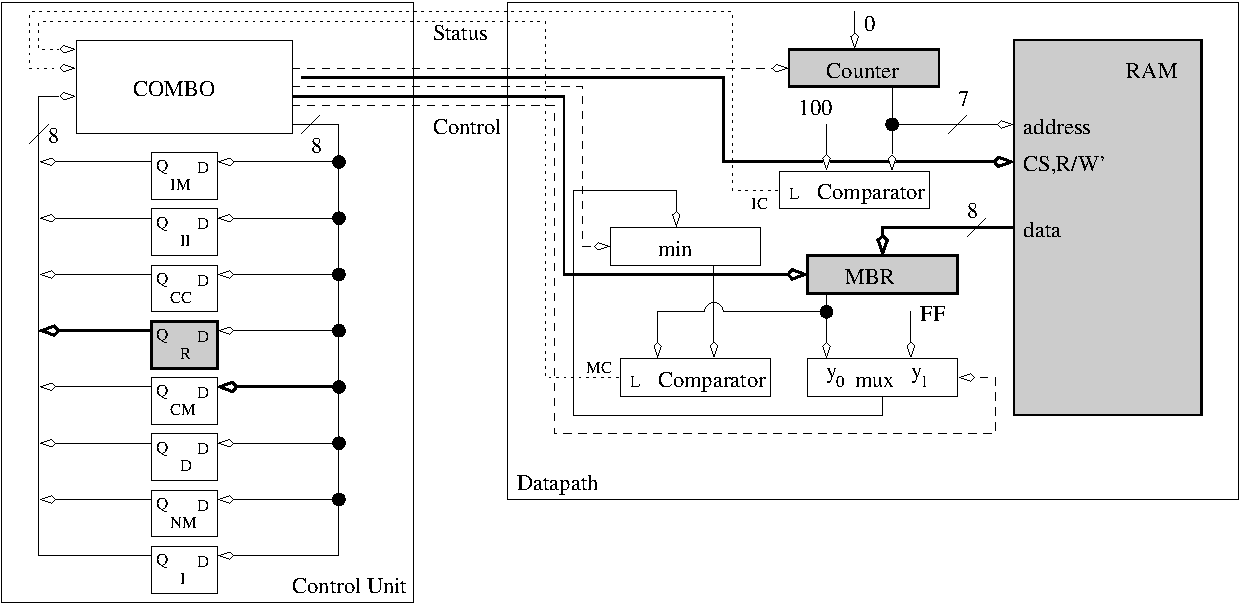
\includegraphics{./Fig8/MinSearch2d}} & 
	\scalebox{0.3}{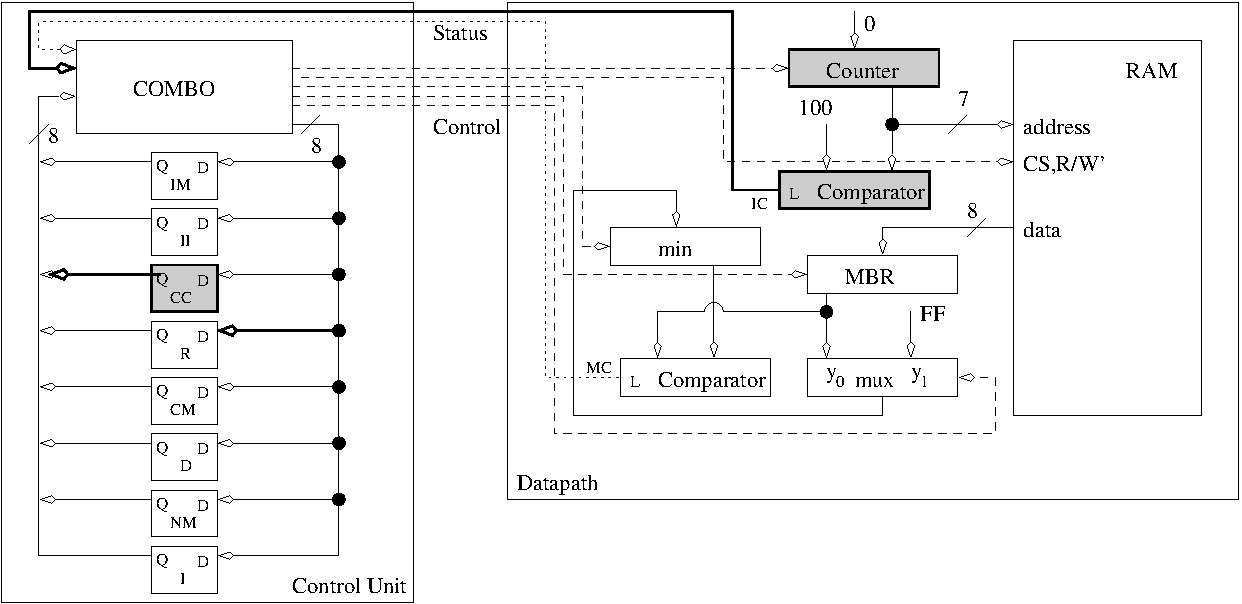
\includegraphics{./Fig8/MinSearch2h}} \\
4. State {\bf Read}                                  & 8. State {\bf CompC} \\
\end{tabular}

\caption{A sequence of figures showing the operation of 
the minimum search circuit through time.  Active components 
are shaded.}
\label{fig:mintable}
\end{figure}

Before moving on with another example, a more
detailed examination of the minimum search circuit's timing
with the goal of determining the maximum clocking frequency
of the circuit is considered.

%% ----------------Timing  -----------------------

\section{Timing}
The timing analysis of a datapath and control circuit is
based on the behavior of the general model of its organization
shown in Figure~\ref{fig:Abstract}.  Since the control unit in
this figure is just a FSM, understanding
the timing analysis of the FSM presented in 
Figure~\ref{fig:GenTime} on page~\pageref{page:GenTime} is imperative.  The goal 
of this analysis is to determine the maximum clock frequency at which
a datapath and control circuit can operate. In order to do 
this, the worst case delay, called the 
critical path, between successive clock edges offers insight.

The positive edge of the clock is used as the reference point
of the timing analysis since this is when the primary source of change
in the circuit, the D flip flops latching their values, occurs.
The positive clock edge has two primary effects: It causes the 
FSM to transition into a new state and it causes the registers in
the datapath to latch new values.  The propagation delay of the
flip flops is referred to as $T_p(A)$ in Figure~\ref{fig:DPTime}.  Since
the datapath requires a valid control word before it can begin, 
the critical path includes the output equation logic. 

The D flip flops which store the state of the control unit's FSM
are the input of the OEs; see Figure~\ref{fig:GenFSM}.  The delay
between the application of a valid $Q$ to when the OEs assert their new
values is referred to as $T_p(B)$ in Figure~\ref{fig:DPTime}.

The OEs of the FSM are the control word of the datapath and
control circuit, telling the elements in the datapath what operation
to perform.  Sequential logic components do not actually
perform their instructed operations until the next clock edge
arrives.  On the other hand, combinational logic components 
perform their operations immediately.  It is easy to construct
datapath instances where the control word effects the status
input to the control unit.  For example, the control word
selects an input of a mux, whose output is routed to a comparator,
whose status output is sent to the control unit.  Thus, the 
combinational logic is on the critical path because its delay 
constrains the maximum clocking frequency.  The time difference 
between the application of a valid control word to the datapath
and the status input to the control unit becoming valid is referred 
to as $T_p(C)$ in Figure~\ref{fig:DPTime}.

The status input to the control unit are routed to the MIE logic;
see Figure~\ref{fig:GenFSM}.  The delay between the status inputs
becoming valid and the MIEs becoming valid is referred to as $T_p(D)$ 
in Figure~\ref{fig:DPTime}.

Once the memory inputs have stabilized, they must be allowed
some setup time, (see page~\pageref{page:setup}), before the next
clock edge.  The setup time is referred to as $T_p(E)$ in 
Figure~\ref{fig:DPTime}.

\begin{figure}[ht]
\center{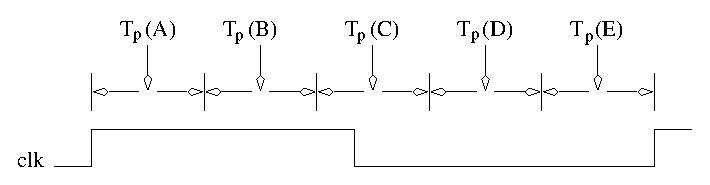
\includegraphics{./Fig8/DPTime}}
\caption{A clock waveform annotated with the delays on the
critical path of a datapath and control circuit.}
\label{fig:DPTime}
\end{figure}
\index{timing!datapath and control}

After the setup time, the outputs of all the circuit elements 
are stable.  Thus, all the flip flops should be ready to latch new 
values on the next clock edge.  Adding together all the
delays on the critical path yields the minimum clocking frequency
$T_{CRITICAL}=T_p(A)+T_p(B)+T_p(C)+T_p(D)+T_p(E)$. The maximum
clocking frequency is the reciprocal of the minimum period.

This timing analysis assumes that there are no combinational devices in 
the datapath requiring more than $T_p(C)+T_p(D)$ time to compute their 
values.  Components like large adders require a lot of time to compute
their values and may exceed these time bounds.  When this happen these 
components become part of the critical path in the timing analysis.

%% -------------------- Parallelism ---------------------------
\subsection{Increasing Parallelism}

Two approaches are used to decrease the amount of time for a 
datapath and control circuit to perform a task: To increase 
the clocking frequency of the circuit, or to decrease the number of
steps required to perform a task.  The first method relies on a
combination of technology and organization of the components in 
the datapath.  The second method relies on increasing the utilization 
of the hardware components in the datapath and consequently decreasing
the number of steps required to perform the task.  
The second approach follows.

In order to have a datapath perform a task in fewer steps, it is
necessary to have the datapath perform multiple steps at the 
same time.  In other words, the goal is to increase the
parallelism of the datapath.  This modification can be done by combining
one or more states of the control unit together.   
Following some common sense rules accomplishes the change.

Two or more assignment statements can be combined if there are 
no conflicts in the hardware resources required for the operations
or if there is no conflict in the order of operations.
For example, the {\bf InitMin} and {\bf InitI} states in the 
minimum search circuit can be performed at the same time because
they operate on separate pieces of hardware.  

Successive ``branches" of the control unit can be combined when
their values are available as shown in Figure~\ref{fig:Branch}.  
In Figure~\ref{fig:Branch}, notice when $X=1$ and $Y=1$,
the control unit moves from state {\bf A} to state {\bf D} via the
state {\bf B}.  If states {\bf B} and {\bf C} do not perform any
operations, then they can be eliminated by transitioning directly
from state {\bf A} to state {\bf D} via an arc labeled $XY$.

\begin{figure}[ht]
\center{\scalebox{0.6}{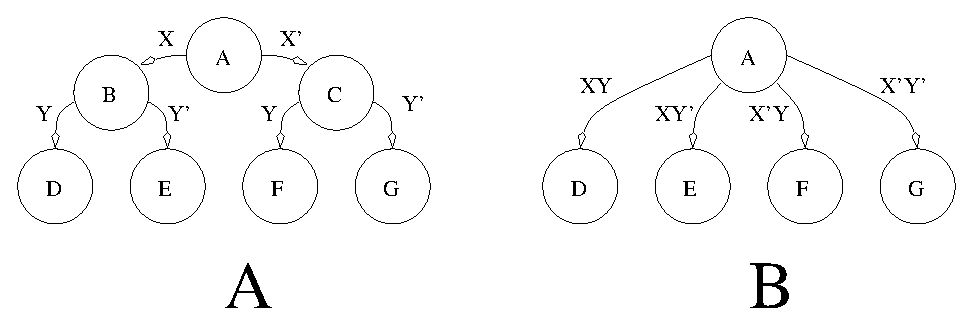
\includegraphics{./Fig8/Branch}}}
\caption{Consecutive branches by the control unit can be combined
using AND.}
\label{fig:Branch}
\end{figure}


%% ---------------- Two-line handshake -----------------------
\section{Two-Line Handshake}
In most cases, digital systems require data from the external world
in order to perform their tasks. In cases where the digital system and
the outside word operate on independent clocks, the transfer of data
is complicated by the lack of a common clock.  To understand how a
reliable transfer of data can be performed in this circumstance, consider the following
scenario of a producer trying to deliver a packet of candies to a
consumer.

Two participants associate in the scenario called {\it producer} and 
{\it consumer}.  The producer has a bag of 32 candies; (the number of 
candies in the bag really does not matter). The candies are to be given to
the consumer and the producer is to receive an acknowledgment from the consumer of their receipt.
Unfortunately, the producer is blind-folded 
and is wearing a rather thick pair of ski mittens so they do not know
when the consumer has actually taken the candies.  The producer and 
consumer must synchronize the transfer of candies using signals sent
with their voices.  The transfer protocol is described in the 
following four steps:

\begin{enumerate}
\item The producer stumbles into consumer's room and calls out, 
``Candies, Candies, $\ldots$"  (non-stop).

\item The consumer gets up, takes the box of candies and then calls
out, ``Received, Received, $\ldots$" (non-stop).  

\item The producer upon hearing the consumer has received the candies
stops calling ``Candies" and walks out of the room. 

\item The consumer upon hearing the producer has stopped 
calling out ``Candies," stops calling out ``Received."
\end{enumerate}

Figure~\ref{fig:ProdConTime} shows a timing diagram for this scenario.
During the time interval labeled 1, both the producer and consumer are
quiet.  Perhaps the producer is negotiating through the 
consumer's rooms.  During time interval 2, the producer is calling out 
and the consumer is quiet.  The consumer, may be busy with some other
task, and is not able to attend to the producer. At the end of time
interval 2, the consumer has taken the candies.  During time interval 3,
perhaps the most annoying time in the scenario, both the producer and
consumer are calling out.  At the end of time interval 3, the producer 
has heard the consumer and is about to stop offering candies.
At the beginning of time 
interval 4, the producer becomes quiet; the producer knows for certain 
the consumer has received the box because the consumer is calling out
``Received."  At the end of time interval 4, the consumer hears the 
producer has stopped calling out ``Candies."  At the beginning of time
interval 5, the consumer stops calling out.  The consumer knows that the
producer knows that the consumer got the box of candies  because the
producer has acknowledged the consumer's thanks by being quiet.

\begin{figure}[ht]
\center{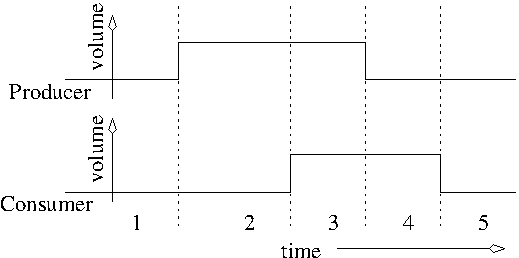
\includegraphics{./Fig8/ProdConTime}}
\caption{A timing diagram of a data transfer between a producer and a consumer.}
\label{fig:ProdConTime}
\end{figure}
\index{timing!producer consumer}

In the above scenario, the producer is the active agent, the
entity initiating the exchange of candies and the consumer is 
the passive agent, the agent that waited for the candies.  This 
protocol, regardless of who is the producer or consumer, is called a 
two-line handshake because the communicating agents must have 
two, coordinating signals, Request (REQ) and Acknowledge (ACK) and at
least one data line.  The REQ signal is used by the active 
agent to signal a readiness to perform a data transfer.  The ACK 
signal is used by the passive agent to acknowledge the data has been 
transferred.  An algorithm description of the two-line handshake for a
digital circuit which is the passive consumer is shown below.

\begin{verbatim}
1.  while(REQ==0);         // Do nothing but wait
2.  register = DATA        // Latch the data
3.  ACK=1;                 // Acknowledge the producer
4.  while(REQ==1);         // Do nothing but wait
5.  ACK=0;                 // Acknowledge the producer
\end{verbatim}

In Line 1 and Line 4, the body of the while loops are empty; there is nothing
to do but wait.  Furthermore, with respect to the external world, (see
Figure~\ref{fig:Abstract}), the ACK and REQ signals act as status and 
command bits, respectively.  The algorithm above is translated into
datapath and control in Figure~\ref{fig:2Line}.

\begin{figure}[ht]
\center{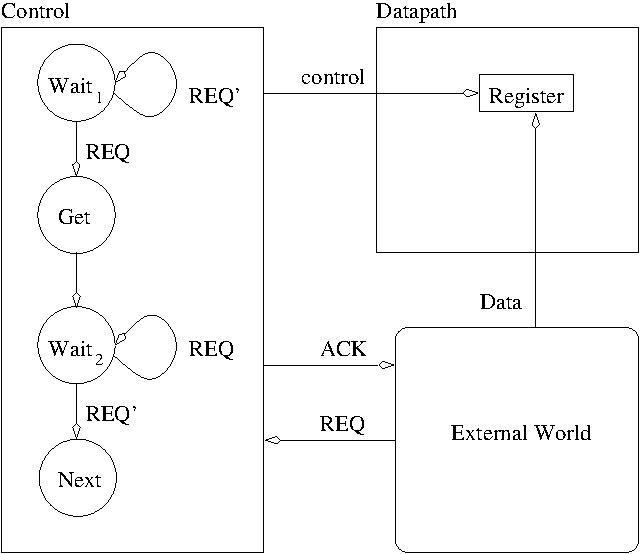
\includegraphics{./Fig8/2Line}}
\caption{The datapath and control components required to implement
a two-line handshake where the digital system is the passive consumer.}
\label{fig:2Line}
\end{figure}

The most important feature of the control unit are the two self-arcs
at states {\bf Wait$_1$ and Wait$_2$}.  In state {\bf Wait$_1$}, the
control unit does nothing except check the value of the REQ signal.
As long as REQ=0, the control unit waits.  As soon as REQ=1,
the control unit proceeds to state {\bf Get} where it enables
the register to load the external data.  The control unit spends a single 
clock cycle in this state before moving to state {\bf Wait$_2$}.  In
state {\bf Wait$_2$}, the control unit asserts and acknowledges,
(ACK=1), and waits for the REQ signal to drop.  It is important
to assert an acknowledge only after latching the data into
the register.  If an acknowledge is sent in the {\bf Get} state,
then it is possible for a very fast external world to be
able to change the data signal before the end of the circuit's 
clock cycle, giving the wrong data.  When the REQ signal is 
dropped, the control unit goes to state {\bf Next} which represents 
some further actions expected of the digital system to perform. In 
state {\bf Next}, (and in all other states except {\bf Wait$_2$}), 
the ACK signal should be set to 0.  

Notice that no matter how different the clock speeds are between the
producer and the consumer, this circuit transfers data correctly.
If the consumer is faster, it will wait patiently for the producer.
If the consumer is slower, it will work as fast as possible to 
latch the data.  

%% ---------------- RAM Counter -----------------------

\section{RAM counter}
The following circuit uses a two-line handshake to transfer a
data item (called the key) to a digital circuit which scans a 
RAM, counting the number of words which match the key.  The word 
statement for this problem is:

\begin{quote}
Build a circuit to read in an 8-bit KEY using a 
two-line handshake; the circuit is a passive consumer.
The circuit should search an 8kx8 RAM, counting the number
of words that match KEY.  Assume the RAM is
preloaded with data and it can respond to a read
request with valid data within one clock cycle.  After 
counting the number of matches, the circuit should wait 
for another key and repeat.
\end{quote}

The algorithm for this circuit needs to read in the key using
a two-line handshake and then needs to read through the RAM, one word
at a time.  Similar to the minimum search algorithm, the
RAM is depicted as an array.  Since it takes a full 
clock cycle to read the
RAM, then it is best to store the currently read word in a 
register for further use.  A register which buffers the contents
of a memory is often called a memory buffer register, or MBR
for short.  Once the RAM value is in the MBR, the value is compared
against the key.  If there is a match, then a register called
match is incremented.

\begin{verbatim}
1.  while(1) {
2.      while(REQ == 0);
3.      KEY = data;
4.      ACK = 1;
5.      while(REQ == 1);
6.      ACK = 0;
7.      match = 0;
8.      for(i=0; i<8191; i++) {
9.          MBR = RAM[i]; 
10.         if (MBR == KEY) {
11.             match=match+1;
12.         } // end if
13.     } // end for 
14. } // end while
\end{verbatim}

{\bf Lines 2-6.} The two-line handshake is formed.  The datapath and control
are similar to Figure~\ref{fig:2Line} with the register being 
named key.

{\bf Line 8.} The for loop generates the address of each word in RAM.  
This line of code adds several states to the control unit and adds
a counter and a comparator to the datapath.  The data output from
the counter provides the address input of the RAM.

{\bf Line 9.} The assignment statement takes the data output from the
RAM and sends it to the MBR register.  While in this state, the 
control unit should read from the memory and assert load on the
MBR's control input.

{\bf Line 10.}  The comparison adds a state to the control unit
in which the E output from the comparator is used in the 
datapath to determine if it should increment the match.

{\bf Line 11.}  The assignment statement increments the number of 
matches if the key is equal to the current memory word.  There
are two reasonable hardware solutions for the match register,
a counter or a register with an adder.  The solution chosen
largely is a matter of preference or of available hardware.
In the solution presented, the register with an adder 
combination is used.  The completed datapath and control is shown in 
Figure~\ref{fig:RAMmatch}.

\begin{figure}[ht]
\center{\scalebox{0.4}{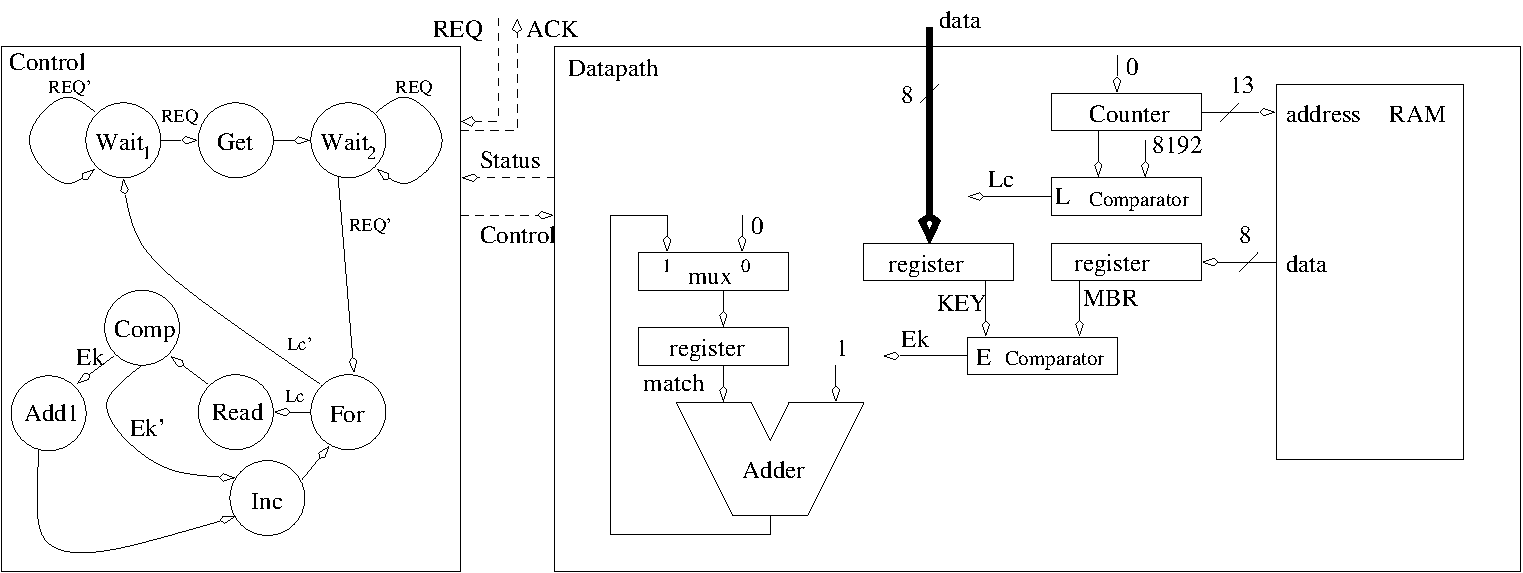
\includegraphics{./Fig8/RAMmatch}}}
\caption{The datapath and control for the RAM match circuit.}
\label{fig:RAMmatch}
\end{figure}

The control word, shown in Table~\ref{table:RAMmatch},
is formed by enumerating the control inputs in the datapath, and by 
listing their values for each state in the control unit.  

\begin{table}
{\tiny
\begin{tabular}{c||c|c|c|c|c|c|c|c}  
{\bf State }  & ACK   & mux       &  Reg match& Reg KEY & Counter     & MBR    & CS       & R/W'    \\ \hline
        & 0     & 0 pass 0  &  0 hold   & 0 hold  & 00 hold     & 0 hold & 0 NULL   & 0 write \\ \hline
        &       &           &           &         & 01 load     &        &          &         \\ \hline
        & 1     & 1 match+1 &  1 load   & 1 load  & 10 count    & 1 load & 1 active & 1 read  \\ \hline \hline
{\bf Wait$_1$ }  & 0     & x         & 0         & 0       & 00          & 0      & 0        & x       \\ \hline
{\bf Get   }  & 0     & x         & 0         & 1       & 00          & 0      & 0        & x       \\ \hline
{\bf Wait$_2$ }  & 1     & x         & 0         & 0       & 00          & 0      & 0        & x       \\ \hline
{\bf match }   & 0     & 0         & 1         & 0       & 00          & 0      & 0        & x       \\ \hline
{\bf Init }   & 0     & x         & 0         & 0       & 01          & 0      & 0        & x       \\ \hline
{\bf For  }   & 0     & x         & 0         & 0       & 10          & 0      & 0        & x       \\ \hline
{\bf Read }   & 0     & x         & 0         & 0       & 00          & 1      & 1        & 1       \\ \hline
{\bf Comp }   & 0     & x         & 0         & 0       & 00          & 0      & 0        & x       \\ \hline
{\bf Inc }    & 0     & 1         & 1         & 0       & 00          & 0      & 0        & x       \\ 
\end{tabular}
}
\caption{The control word for the RAM match circuit and its value for each state.}
\label{table:RAMmatch}
\end{table}


%% -------------------------Keyboard --------------------

\section{Keyboard Scancode Reader}
Even though PS/2 keyboards are being replaced with their USB counterparts,
they are still a common piece of technology that can easily be incorporated 
into digital systems with the help of a scan code reader.  Before building
a scan code reader, understanding how a keyboard works must come first.
Using the input, output, and behavior tables utilized
in Chapters 4 and 6 supports this goal.

\begin{tabular}{|l|p{3.5in}|} \hline
Nomenclature:  & PS/2 Keyboard				\\ \hline
Data Input:    & none					\\ \hline
Data Output:   & 1-bit data, nominally logic 1		\\ \hline
Control:       & none					\\ \hline
Status:        & none					\\ \hline
Others:        & 1-bit clk, nominally logic 1		\\ \hline
Physical Input:& key press and key release events 	\\ \hline
Physical Output:& none		\\ \hline
Behavior:      & When a key is pressed, its 8-bit make code
		is transmitted.  When a key is released, an
		8-bit break code is transmitted, immediately
		followed by the key's 8-bit scan code.	\\ \hline
\end{tabular}

While the table implies a keyboard is an output-only device, the
truth is the clock and data lines are open collector signals.  In other words, 
the clock and data lines can safely be manipulated by the 
external world to configure a keyboard.  A common example of such 
bidirectional communication occurs every time the
``Caps Lock" key is pressed on a keyboard.  When this happens, the keyboard 
sends the ``Caps Lock" scan code to the PC and the PC in return writes 
a ``Toggle Caps Lock LED" command to the keyboard.  Since the keyboard 
scan code reader does not write to the keyboard, it assumes that the
clock and data signals are outputs from the keyboard.

When a keyboard key is pressed, the keyboard sends one 
packet of information as shown at the top of Figure~\ref{fig:Keyboard}.
The 8-bit data contained in this make code is the scan code of the 
key pressed.  The relationship between the keys and their scan codes
is not at all obvious and is not based on ASCII. The exact codes are
immaterial to the discussion; the curious reader can perform a quick 
Internet search on ``PS/2 keyboard scan codes" to get a complete listing.
When a key is released, two packets are transmitted as shown at the 
top of Figure~\ref{fig:Keyboard}.  The break code is almost always 
equal to 0xF0.  The final packet is the scan code of the released 
key.  

While there is a scan code for ``a" key, there is not a scan code
for ``A".  The device reading the keyboard interprets the make code
for ``shift," and then sees a make code for ``a".  From this, the device
reading the keyboard should understand that the user wants a capital
``A".  More than likely, the user will release the ``a", first causing 
its break code and scan code to be transmitted, followed by the break
and scan code for the ``shift" key.

Each of these packets consists of 11 bits as shown in the lower half 
of Figure~\ref{fig:Keyboard}.  The data from the keyboard is always 
valid on the falling edge of the clock signal.  The keyboard asserts
new data on or around the rising edge of the clock.  The 11-bit data 
packet always begins with a start bit equal to 0.  Following the
start bit are 8-bits of data, transmitted least-significant bit first.
Following the data bits is an odd-parity bit, whose value is set by the 
keyboard so that the total number of 1s transmitted in the eight data
bits plus the parity bit equals an odd number.  For example, if the
eight data bits are 01100011, then the parity bit would equal 1 so that 
the total number of 1s would be an odd number, in this case 5.  By
adding some additional circuitry, the parity bit can be used to detect 
errors in transmission.   Following the parity bit, the final bit of
the data packet, the stop bit, is sent and is always equal to 1.

\begin{figure}[ht]
\center{\scalebox{0.7}{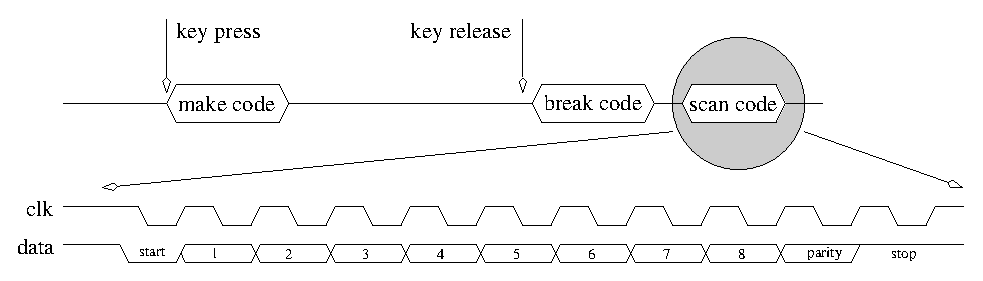
\includegraphics{./Fig8/Keyboard}}}
\caption{The behavior of the keyboard clock and data lines to a 
key press event.}
\label{fig:Keyboard}
\end{figure}

The keyboard scan code reader circuit assumes only one key is
pressed at a time.  That is, while a key is being held down,  
no other key is assumed to be pressed.  Thus, typing in ``A" may 
result in the keyboard scan code reader generating an invalid output. 
Furthermore, the circuit ignores the parity bit, forgoing any 
possibility of checking for errors in the transmitted data.  The
input, output, and behavior of the keyboard scan code reader is
summarized in the following table.

\begin{tabular}{|l|p{3.5in}|} \hline
Nomenclature:  & Keyboard scan code reader		\\ \hline
Data Input:    & 1-bit kd\_data, nominally logic 1
		 1-bit kd\_clk, nominally logic 1	\\ \hline
Data Output:   & 8-bit scan code				\\ \hline
Control:       & none					\\ \hline
Status:        & 1-bit busy, nominally logic 0		\\ \hline
Others:        & 1-bit clk, nominally logic 1		\\ \hline
Behavior:      & Interprets the PS/2 keyboard clk and data signal
		from a keypress event and outputs the associated
		scan code.  The busy signal goes high when the
		first data bit arrives and stays high until the
		last data bit is received.  Busy is low only when
		there is a valid scan code on the output. \\ \hline
\end{tabular}
\\ \\
The keyboard scan code reader algorithm just shifts in the 33 bits
sent from the keyboard and holds the busy signal high while doing 
this.  The scan code is extracted from the low-order bits of the shift
register outputs.

\begin{verbatim}
1.  while(1) {
2.      busy=0;
3.      while (kb_clk == 1);
4.      busy=1;
5.      for (count=0 count<33; count++) {
6.          while(kb_clk == 1);
7.          shift = (shift << 1) | kb_data;
8.          while(kb_clk == 0);
9.      } 
10.     scan = shift[9-2]
11. } 
\end{verbatim}

Note the keyboard clock, kb\_clk, signal is being treated as an ordinary 
data input signal, rather than as a clock signal.  This decision seems to 
increase the complexity of the solution, but actually makes implementing 
the circuit easier on FPGAs because the clock does not require special 
clock net resources and it makes integrating
clock debouncing circuits easier.  The keyboard scan algorithm is converted
into datapath and control by parsing it line-by-line.

{\bf Line 1.} The while loop formed by Line 1 and Line 9 means the scan code reader 
is expected to operate forever.	This statement is responsible for the 
{\bf start} state in Figure ~\ref{fig:kbscan}.

{\bf Line 2.} The assignment statement can be handled with the control unit
because busy is a single bit.  Thus, the assignment state does not introduce
any states in the control unit.

{\bf Line 3.} The delay loop waits for the falling edge of the keyboard clock.
Introducing a 1-bit comparator in the datapath to check if kb\_clk is equal
to 1 is wasteful because the E output of the comparator is equal to kb\_clk
itself.  Hence, the kb\_clk signal is sent directly to the control unit as
a status signal.  The while loop is responsible for the {\bf while} state 
in Figure ~\ref{fig:kbscan}.

{\bf Line 4.} The statement is incorporated into the control word.  Its
value is assigned in the states which make up the surrounding statements.

{\bf Line 5.} This line of code requires  a 6-bit counter and a 6-bit 
comparator to be added to the datapath.  The statement is responsible 
for the {\bf clear}, {\bf inc} and {\bf done?} states in 
Figure ~\ref{fig:kbscan}.  Note that the {\bf done?} state closes the 
infinite loop started in Line 1.

{\bf Line 6.} The delay loop in Line 3 is used to distinguish the start of a 
keypress event and consequently, when to set the busy bit to 1.  The 
delay loop on Line 6 indicates the presence of a negative edge on the 
keyboard clock and hence a valid data bit.  This statement is responsible 
for the {\bf wait1} state in Figure ~\ref{fig:kbscan}.

{\bf Line 7.} In order to get to Line 7, a negative edge on kb\_clk occurred.
Hence, the keyboard data is latched up into a shift register.  This 
statement is responsible for the {\bf shift} state in Figure ~\ref{fig:kbscan}.

{\bf Line 8.} A delay loop is waiting for the rising edge of the keyboard clock.  
As with Line 3 and Line 6, this statement requires no hardware in the datapath.  
The statement is responsible for the {\bf wait0} state in Figure ~\ref{fig:kbscan}.

\begin{figure}[ht]
\center{\scalebox{0.7}{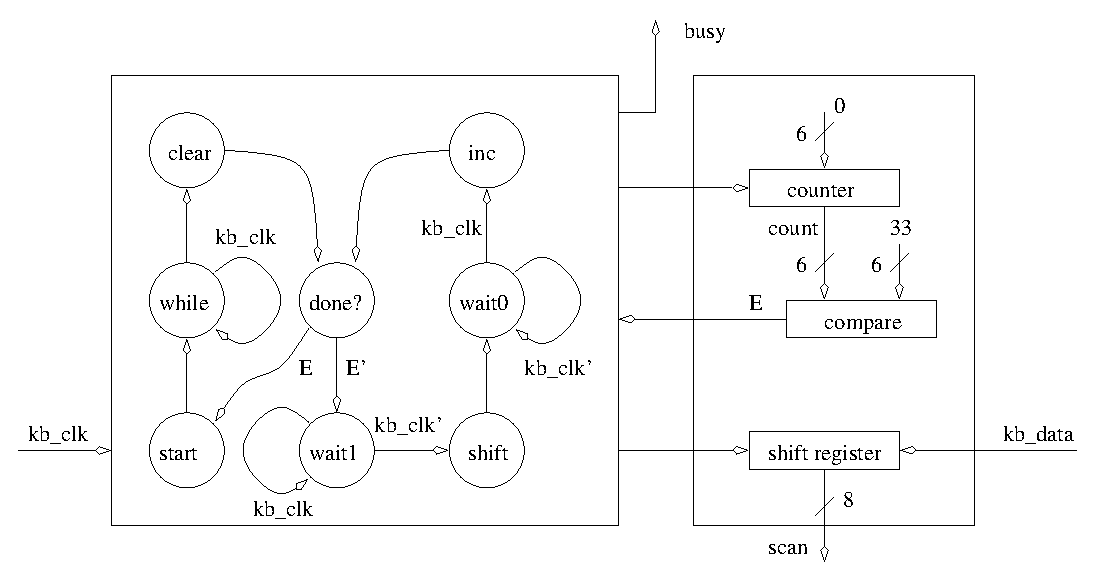
\includegraphics{./Fig8/Kbscan}}}
\caption{The datapath and control for the kbscan circuit.}
\label{fig:kbscan}
\end{figure}

The control word is formed by writing down the control settings for 
all the components in the datapath.  Next, each state is listed, each 
in its own row, and the binary control word for each state is defined
in Table~\ref{table:kscan}.

\begin{table}
\begin{tabular}{c||c|c|c}  
{\bf State }  & Counter	& Shift Reg	&  Busy  		\\ \hline
        & 00 hold	& 00 hold	& 0 valid output	\\ \hline
        & 01 load	& 01 load	& 1 invalid output	\\ \hline
        & 10 count	& 10 shift left	& 			\\ \hline
        &      		& 11 shift right&			\\ \hline \hline
{\bf start }	&	01	&	00	&	0	\\ \hline
{\bf while }	&	00	&	00	&	0	\\ \hline
{\bf start }	&	00	&	00	&	0	\\ \hline
{\bf clear }	&	01	&	00	&	1	\\ \hline
{\bf done? }	&	00	&	00	&	1	\\ \hline
{\bf wait1 }	&	00	&	00	&	1	\\ \hline
{\bf shift }	&	00	&	11	&	1	\\ \hline
{\bf wait0 }	&	00	&	00	&	1	\\ \hline
{\bf inc }	&	10	&	00	&	1	\\ 
\end{tabular}
\caption{The control word for the keyboard scan circuit and its values for each state.}
\label{table:kscan}
\end{table}

This concludes the construction of the keyboard scan code reader circuit.
The circuit, however, is used in the following section in order to build a
circuit to generate a light show.

%% ---------------- Light Show -----------------------

\pagebreak
\section{Light Show}

A light show consists of an endlessly repeating sequence of up to 16 frames. 
A frame is an illuminated pattern of LEDs on a LED bar graph. The user 
creates a light show by specifying the number of frames in the show, editing 
those frames, and then instructing the circuit to cycle through the frames. 
The input to the circuit comes from a standard PS/2 keyboard. The output of 
the circuit is displayed on a LED bar graph and a 7-segment display. The 
behavior of the Light Show circuit is given in Figure~\ref{fig:LSbehavior}.
 
\begin{figure}[ht]
\center{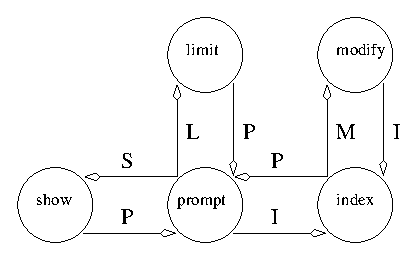
\includegraphics{./Fig8/Behavior}}
\caption{A state diagram describing the behavior of the Light Show circuit.}
\label{fig:LSbehavior}
\end{figure}

The Light Show circuit changes state when the users presses a key on 
the keyboard. For example, pressing ``M" while in the {\bf index } state causes 
the circuit to transition into the {\bf modify state}. The behavior of the 
Light Show circuit in each of its states is described in 
Table~\ref{table:LSbehavior}.

\begin{table}
\begin{tabular}{l|l|l|p{2.0in}}
{\bf State }	& LED bar graph	& 7-segment	& Behavior 				\\ \hline \hline
{\bf reset }	& blank		& blank		& All sequential elements are reset 	\\ \hline
{\bf prompt }	& blank		& ``P"		& Waiting for user input		\\ \hline
{\bf limit }	& blank		& current limit	& The number of frames in the light show is called 
	the limit. If the user enters a hex value between 0-F it is stored as the new limit. \\  \hline
{\bf index }	& current frame	& current index	& Each frame in the show has an index which defines 
	its position in the show. If the user enters a hex value between 0-F, this frame will 
	be edited in the {\bf modify } state. 						\\ \hline
{\bf modify }	& current frame	& current index	& Each frame has eight bits which specify the state of 
	the 8 LEDs on the bar graph.  These bits are toggled by pressing the corresponding 
	key. For example, if LED 5 is on, pressing ``5", causes LED 5 
	to go off.								\\ \hline
{\bf show }	& cycle through frames & current index & Consecutive frames are displayed on the 
	LED bar graph at around 4Hz. After the last frame is displayed, the circuit loops 
	back to the 0th frame. 							\\ 
\end{tabular}
\caption{The behavior of the Light Show circuit in each of its states.}
\label{table:LSbehavior}
\end{table}

The algorithm for the light show circuit continually scans the busy signal 
and the keyboard scan code.  When the user presses either a ``L", 
``I", or ``S", 
the algorithm drops into one of the subfunctions described in 
Table~\ref{table:LSbehavior}.  Assume the Light Show circuit is
clocked at 16MHz.  The clock rate is needed in order to create a delay of
0.25 seconds required to pace the frames during the show phase.  The delay is
created by having the circuit wait for a counter to count up from 0 to 
4,000,000.  The function calls in the algorithm are explained in the 
subsequent line-by-line analysis.

\pagebreak
\begin{verbatim}
1.  while(1) {
2.      HexDisplay = ``P"
3.      if (!busy and IsL(ScanCode)) {
4.          while (!busy' and !IsP(ScanCode)) {
5.             HexDisplay = Hex2Seven(limit);
6.             BarGraph = 0x00;
7.             if (!busy and IsHex(ScanCode)) {
8.                  limit = Scan2Hex(ScanCode);
9.                  while(!busy);
10.     }   }  }

11.     if (!busy and IsI(ScanCode)) {
12.         while (busy or !IsP(ScanCode)) {
13.             HexDisplay = Hex2Seven(index);
14.             if (!busy and IsHex(ScanCode)) {
15.                index = Scan2Hex(ScanCode);
16.                 while(!busy);
17.             }

18.             if (!busy and IsM(ScanCode)) {
19.                 while (busy or !IsI(ScanCode)) {
20.                     HexDisplay = Hex2Seven(index);
21.                     BarGraph = RAM[index];
22             	        while(!busy);
23             	        while(busy);
24.                     if (!busy and IsOct(ScanCode)) {
25.                         RAM[index] = Flip(IsOct(ScanCode),RAM[index]);
26.	}   }   }   }   }

27.     if (!busy and IsS(ScanCode)) {
28.	    index = 0;
29.         while(!busy and !IsP(ScanCode)) {
30.             BarGraph = RAM[index];
31.             HexDisplay = Hex2Seven(index);
32.             for (timer=0; timer<2^22; timer++);
33.             index += 1;
34.             if (index == limit) index=0;
35.  }  }   }
\end{verbatim}

As each line is parsed, new states are added to the control unit and basic building 
blocks are added to the datapath.  In several cases, brand new building blocks need 
to be created in order to perform the tasks required of the datapath.  Descriptions of
these components are provided, but the structure of their internal organization 
is left to the reader to determine.

{\bf Line 1.} The infinite loop formed by Line 1 and Line 35 means that the outermost loop 
in the control unit cycles in the {\bf prompt} state in Figure~\ref{fig:LightShowCir} 
until something happens.

{\bf Line 2.} From the word statement, the 7-segment display shows ``P" or a numerical value.
A 2:1 mux in the datapath resolves this conflict. Since the assignment statement
is performed without the need to actually assign a value to a register, no 
explicit state is required.  The control unit selects the ``P" input when in the 
{\bf prompt} state.  

{\bf Line 3.} The busy signal is generated by the kbscan component in the datapath.  
The functional notation ``IsL(ScanCode)" is just short-hand for the IsL output from 
the ScanDecode component in the datapath.  The ScanDecode component takes in the
8-bit scan code from the kbscan component and outputs 1 when the scan code corresponds
to the scan code for the letter ``l".  The ANDing of busy' and IsL signals is handled 
by the internal logic in the control unit.  When the condition is true, the control 
unit transitions to the {\bf set limit} state.

{\bf Line 4.} The condition of the while statement is checked in the {\bf set limit} 
state.  When the user presses a ``p" in the {\bf set limit} state, the control 
unit transitions back to the {\bf prompt} state.  See page \pageref{page:IsScan}
for more details regarding the scan code recognizer circuit.

{\bf Line 5.} Two different numerical values can be displayed on the 
7-segment display, limit and index (Line 13).  The 2:1 multiplexer in front of 
the Hex2Seven component allows the control unit to select which of these two values is 
converted and sent onto the display.  The control unit asserts its control 
outputs to route the limit register's output to the 7-segment display in 
the {\bf set limit} state.

{\bf Line 6.} The LED bargraph displays two different values on its output, 0x00 and 
RAM[index], (Line 21).  The 2:1 multiplexer placed in front of the LED bargraph 
resolves this conflict.  The control unit selects 0x00 when it is in the 
{\bf set limit} state.

{\bf Line 7.} If the control unit detects a hexadecimal character has arrived while 
in the {\bf set limit} state, the control unit transitions to the {\bf load 
limit} state.  The datapath already contains the hardware necessary to check 
this condition.

{\bf Line 8.} This assignment is performed in the {\bf load limit} state where the control 
unit asserts a load command to the limit register.  The data input to the limit 
register comes from the converted scan code via the Scan2Hex component.  The Scan2Hex
component takes in an 8-bit scan code corresponding to a key representing a hexadecimal
character and converts it into its 4-bit value. See page \pageref{page:ScanDecode}
for more details.

{\bf Line 9.}  After loading the limit register, the control unit immediately transitions 
to the {\bf wait limit} state.  Then, the control unit waits for some keyboard activity 
before transitioning back to the {\bf set limit} state.  This action is done in order to prevent 
the limit register from being continuously loaded while waiting for keyboard activity.
Such repetitive loading is considered bad form.  While waiting in this state the control 
unit should display the new limit register on the 7-segment display.

{\bf Line 10.} The If/Then statement started on Line 3 is terminated.

{\bf Line 11.} This statement causes the control unit to transition to the {\bf set index}
 state.

{\bf Line 12.} The while statement returns the control unit transition to the {\bf prompt} state when 
``p" is pressed.

{\bf Line 13.} When the control unit is in the {\bf set index} state, the 7-segment display 
should show the current index by asserting the correct control signals.

{\bf Line 14.} When the control unit is in the {\bf set index} state and a hexadecimal 
character is typed, the control unit should transition to the {\bf load index} state.

{\bf Line 15.} Since the primary purpose of the index is to walk through the memory 
during a light show, it is stored in a counter.  The control unit signals the 
counter to load the index in the {\bf load index} state.

{\bf Line 16.} After loading the index register, the control unit transitions to the {\bf wait 
limit} state where it waits for keyboard activity before transitioning back 
to the {\bf set index} state.

{\bf Line 17.} Closes the if/then statement from Line 14.

{\bf Line 18.} When the control unit is in the {\bf set index} state, a keypress of ``m" 
causes it to transition to the {\bf modify} state.

{\bf Line 19.} When the control unit is in the {\bf modify} state, a keypress of ``i" 
causes it to transition to the {\bf set index} state.  Otherwise the control 
unit transitions to the {\bf read} state.  

{\bf Line 20.} When in the {\bf read} state, the control unit should route the current 
index to the 7-segment display.

{\bf Line 21.} When in the {\bf read} state the control unit instructs the bargraph register 
to load the current frame from the RAM.


{\bf Line 22.} After reading the current frame, the control unit transitions 
to the {\bf wait! busy} state where it displays the frame on the LED bargraph 
and waits for a keypress event.

{\bf Line 23.} The control unit waits for a key press event in order 
to leave the {\bf wait busy} state.

{\bf Line 24.} If the keypress event was an octal digit, the control 
unit transitions to the {\bf write} state, otherwise it goes to the 
{\bf modify} state to check if the keypress was an ``i".

{\bf Line 25.}  In the {\bf write} state, one of the current frame's 
bits are flipped and then the altered frame is stored back into the 
RAM.  The lower three bits of the converted scan code tell the flip 
component which bit of the frame to invert.  Refer to 
page \pageref{page:flipbox} for further details regarding the flip 
component.  After this, the control unit goes to the {\bf read} state 
which started the while loop on Line 19.

{\bf Line 26.} The preceding control structures are terminated, ending with the if/then on Line 11.

{\bf Line 27.} This statement causes the control unit to transition to the 
{\bf reset index} state.

{\bf Line 28.} When in the {\bf reset index} state, the control unit instructs the index 
counter to synchronously reset its value to 0.

{\bf Line 29.} Pressing ``p" stops the light show and returns the control unit to the 
{\bf prompt} state.  This check is performed during the first state, {\bf load frame}, 
of the while loop.

{\bf Line 30.} The bargraph register is loaded with the current frame during the 
{\bf load frame} state.

{\bf Line 31.} The control unit should display the current index on the 7-segment display 
during all the states which make up the while loop of the light show.  In preparation for 
the loop in the next line, the timer counter is reset to 0 in the {\bf load frame}
 state.

{\bf Line 32.} In the {\bf wait frame} state, the control unit increments the 
delay counter from 0 to 4,000,000.  The comparator on the delay counters output 
signals to the control unit when this happens.  Since the clock is running at 
16MHz, this count value will hold the control unit in the {\bf wait frame} state
for 1/4 of a second.

{\bf Line 33.}  When in the {\bf inc index} state, the control unit increments 
the index of the current frame.

{\bf Line 34.} When the control unit is in the {\bf comp index} state, it checks 
the index equals the limit.  If it does, the control unit transitions to 
the {\bf reset index} state, otherwise the next frame is loaded in the 
{\bf load frame} state.

{\bf Line 35.}  The program is closed.

The net accumulation of the states and hardware added in the parsing of the Light Show 
algorithm are shown in Figure~\ref{fig:LightShowCir}.
 
\begin{figure}[ht]
\center{\scalebox{0.6}{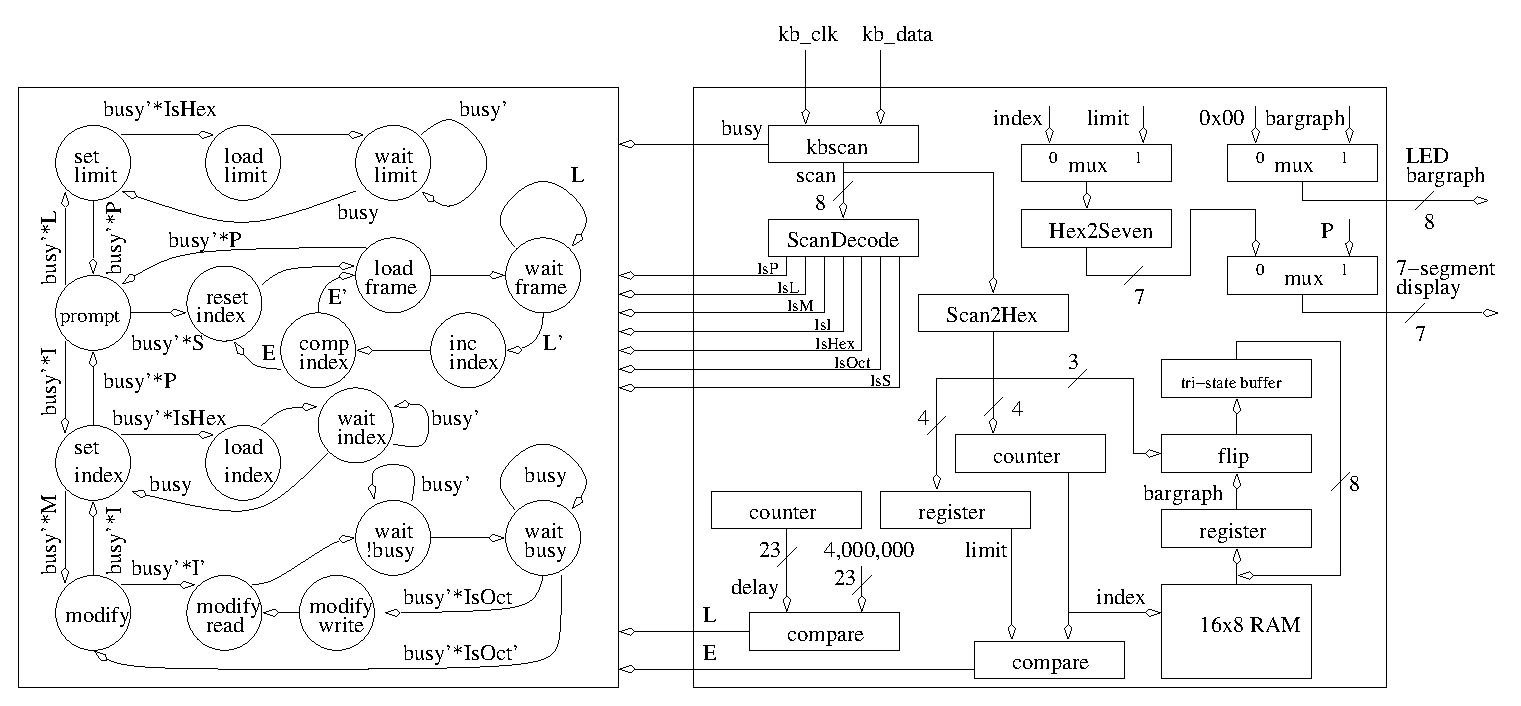
\includegraphics{./Fig8/LightShowCir}}}
\caption{The datapath and control for the Light show circuit.}
\label{fig:LightShowCir}
\end{figure}

The next step in the design of Light Show circuit is to define the control word and 
its value for each of the states shown in Figure~\ref{fig:LightShowCir}.  The control 
word is the set of signals from the control unit to the control inputs of the 
components in the datapath.  The top row of Table~\ref{table:LightShow} lists all 
the components in the datapath which have control inputs.  The resulting 11-bit control 
word is then defined for each of the 17 states. The actions performed in each state 
are determined from the line-by-line analysis of the light show algorithm.

\begin{table}
{\tiny
\begin{tabular}{c||c|c|c|c|c|c|c|c|c|c|c}
{\bf State } 	& bar & 7-seg & hex & index & delay & limit    & bargraph & CS & R/W' & tsb & flip \\  
	& mux & mux   & mux & count & count & register & register &       &       & &      \\  \hline \hline
	& 0 0x00 & 0 index & 0 7-seg & 00 hold & 00 hold & 0 hold & 0 hold & 0 off & 0 write & 0 tri & 0 pass \\ 
	& 1 bar	& 1 limit & 1 ``P"& 01 cnt & 01 cnt & 1 load &    1 load & 1 on    &  1 read & 1 pass & 1 flip \\
	& 	&     &     & 10 load & 10 load & & & & & \\
	& 	&     &	    & 11 reset	& 11 reset & & & & \\ \hline \hline
{\bf prompt } 	 & 	0 &	x &	1 &	00 &	00 &	0 &	0 &	0 & x &	0 & x \\ \hline
{\bf set limit }  & 	0 &	1 &	0 &	00 &	00 &	0 &	0 &	0 & x &	0 & x \\ \hline
{\bf load limit } &	0 &	1 &	0 &	00 &	00 &	1 &	0 &	0 & x &	0 & x \\ \hline
{\bf waitlimit } &	0 &	1 &	0 &	00 &	00 &	0 &	0 &	0 & x &	0 & x \\ \hline
{\bf reset index } &	1 &	0 & 	0 &	11 &	00 &	0 &	0 &	0 & x &	0 & x \\ \hline
{\bf load frame } &	1 &	0 &	0 &	00 &	11 &	0 &	1 &	1 & 1 & 0 & x \\ \hline
{\bf wait frame } &	1 &	0 &	0 &	00 &	01 &	0 &	0 &	0 & x &	0 & x \\ \hline
{\bf inc index } &	1 &	0 &	0 &	01 &	00 &	0 &	0 &	0 & x &	0 & x \\ \hline
{\bf comp index } &	1 &	0 &	0 &	00 &	00 &	0 &	0 &	0 & x &	0 & x \\ \hline
{\bf set index } &	0 &	0 &	0 &	00 & 	00 &	0 & 	0 &	0 & x &	0 & x \\ \hline
{\bf load index } &	0 &	0 & 	0 &	10 &	00 &	0 &	0 &	0 & x & 0 & x \\ \hline
{\bf wait index } &	0 &	0 &	0 &	00 &	00 &	0 &	0 &	0 & x &	0 & x \\ \hline
{\bf modify	} &	0 &	0 &	0 &	00 &	00 &	0 &	0 &	0 & x &	0 & x \\ \hline
{\bf modify read} &	1 &	0 &	0 &	00 &	00 &	0 &	1 &	1 & 1 &	1 & x \\ \hline
{\bf modify write } &	1 &	0 &	0 &	00 &	00 &	0 &	0 & 	1 & 0 &	0 & 1 \\ \hline
{\bf wait !busy } &	1 &	0 &	0 &	00 &	00 &	0 &	0 &	0 & x &	0 & x \\ \hline
{\bf wait busy } &	1 &	0 &	0 &	00 &	00 &	0 &	0 &	0 & x &	0 & x \\ 
\end{tabular} 
}
\caption{The control word for the LightShow circuit and its value for each state.}
\label{table:LightShow}
\end{table}

The reader is left to derive the MIEs and OEs for the control unit.
\section{Exercises}
\section{Exercises}
\label{section:datapathControl}
\graphicspath{ {./chapter08/FigHw} }

\begin{enumerate}
\item \textbf{ (4 pts.)}
Show how to eliminate the 4-bit 2:1 mux in the bit counter by
assuming that the Y register had an asynchronous active low reset input.
Consider the fact that the external world still needs the ability to hit
a single button to reset the state of the entire circuit. 

\item  \textbf{ (6 pts.)}
A control unit has been built with the following control word:

\begin{tabular}{|c|c|c|c|c|}  \hline
Reg A       & Reg B         &  Reg P        & P mux         \\ \hline
00 hold     & 00 hold       &  1 hold       & 1 Load 0      \\ \hline
11 lsr      & 11 lsr        &               &               \\ \hline
10 lsl      & 10 lsl        &  0 load       & 0 Load Add    \\ \hline
01 load     & 01 load       &               &               \\ \hline 
\end{tabular}

Regrettably, these setting were completely wrong.  In reality here is what the control word should
have been:

\begin{tabular}{|c|c|c|c|c|}  \hline
Reg A       & Reg B         &  Reg P        & P mux         \\ \hline
00 hold     & 00 hold       &  0 hold       & 0 Load 0      \\ \hline
01 lsr      & 01 lsr        &               &               \\ \hline
10 lsl      & 10 lsl        &  1 load       & 1 Load Add    \\ \hline
11 load     & 11 load       &               &               \\ \hline 
\end{tabular}

The design team is in a total panic.
The design team thinks that it will take weeks to straighten out the error, 
they claim that the control unit needs to be redesigned.  However, there is
a cheap and easy solution.  Design some combinational 
logic to insert between the faulty control unit and the datapath in order
to straighten out the bum control signals.  There is one error can be 
fixed by changing something in the datapath, no extra hardware is 
required.  Identify this error and its solution.

\item \textbf{ (8 pts.)}
Modify the algorithm for the bit counting circuit so that it uses a 
two-line handshake to transmit the Y register.  The circuit should take
the role of an active producer in the transmission of Y.  The circuit
has four handshaking lines and two data lines.  Hint, a common
error of students is to insert a three-state buffer on the output of
the Y register to the outside world to prevent its transmission to
the outside world until the value of Y is finalized.  Don't do this!
If the outside world reads the value of Y before the circuit's signals
are valid (via the send\_REQ signal) then its their own dumb fault.
Just send the Y signal outside the datapath as is.

\item \textbf{ (16 pts.)} 
A 8kx32 RAM is full of integer data.  Design a circuit to scan
the RAM and find its smallest value.  

Turn in; an algorithm the datapath and control unit, the control word 
table, the memory input equations, and output equations.  
The control unit is to be implemented using a ones hot encoding.


\item \textbf{ (16 pts.)}
A 8kx32 RAM is full of integer data.  Design a
circuit that determines the sum of the integers {\em between} addresses
A and B.  The values of A and B are to be read in using a two-line
handshake where the circuit is to act as a passive consumer.  
The sum is to be placed in a 32-bit register S.
Turn in; an algorithm the datapath and control unit, the control word 
table, the memory input equations, and output equations.  
The control unit is to be implemented using a ones hot encoding.

\begin{onlysolution}  \textbf{Solution} \itshape{

\textbf{ Algorithm}

while(REQ==0); \\
A = datain; \\
ACK=1; \\
while(REQ==1); \\
ACK=0; \\
while(REQ==0); \\
B = datain; \\
ACK=1; \\
while(REQ==1); \\
ACK=0; \\
S=0; \\
for(i=A; i<B; i++)  { \\
 MBR=RAM[i]; \\
 S=S+MBR; \\
} // end for \\

\textbf{ DP \& CU}

\begin{figure}[ht]
\center{\scalebox{0.7}{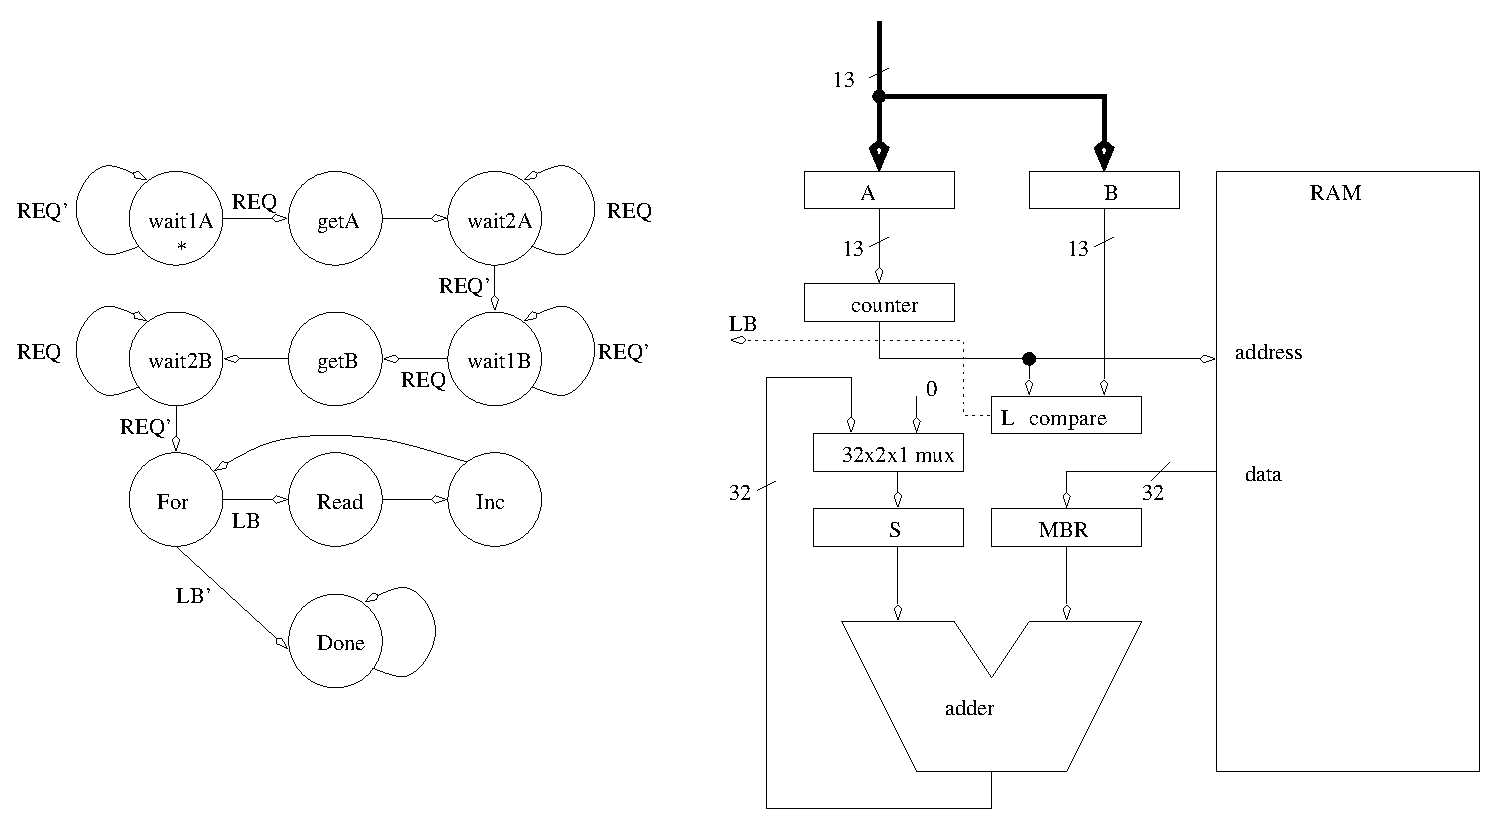
\includegraphics{Sol8-5}}}
\caption{The datapath and control to determine the sum between
addresses A and B.}
\end{figure}


\textbf{ Control Word}

\begin{tabular}{l|l|l|l|l|l|l}
STATE & A      & B      &MUX          &S      &MBR    &counter	\\ \hline
      & 0 hold & 0 hold &0 pass 0     &0 hold &0 hold &00 hold	\\ \hline
      & 1 load & 1 load &1 pass S+MBR &1 load &1 load &01 UP	\\ \hline
      &        &        &             &       &       &10 load	\\ \hline
Wait1A& 0      & 0      &0            &0      &0      &00	\\ \hline
GetA  & 1      & 0      &0            &0      &0      &00	\\ \hline
Wait2A& 0      & 0      &0            &0      &0      &00	\\ \hline
Wait1B& 0      & 0      &0            &0      &0      &00	\\ \hline
GetB  & 0      & 1      &1            &1      &0      &10	\\ \hline
Wait2B& 0      & 0      &0            &0      &0      &00	\\ \hline
For   & 0      & 0      &0            &0      &0      &00	\\ \hline
Read  & 0      & 0      &0            &0      &1      &01	\\ \hline
Inc   & 0      & 0      &1            &1      &0      &00	\\ \hline
Done  & 0      & 0      &0            &0      &0      &00	\\ 
\end{tabular}

\textbf{ MIEs and OEs}

\begin{tabular}{ll}
MIE					&	OE			\\
$D_{Wait1a}= Q_{wait1a}req'$		&  $Z_{A} = Q_{getA}$		\\
$D_{GetA } = Q_{wait1a}req$		&  $Z_{B} = Q_{getB}$		\\
$D_{wait2a}= Q_{getA} + Q_{wait2A}req$	&  $Z_{MUX} = Q_{getB} + Q_{Inc}$		\\
$D_{wait1b}= Q_{wait2a}req' + Q_{wait1B}req'$	&  $Z_{S} = Q_{getB} + Q_{Inc}$		\\
$D_{GetB } = Q_{wait1b}req$		&  $Z_{MBR} = Q_{Read}$		\\
$D_{wait2B}= Q_{GetB} + Q_{wait2b}req$	&  $Z_{c1} = Q_{GetB}$		\\
$D_{For  } = Q_{wait2B}req'$		&  $Z_{c0} = Q_{Read}$		\\
$D_{Read } = Q_{For}LB$			&  		\\
$D_{Inc  } = Q_{Read}$			& 		\\
$D_{Done } = Q_{For}LB'$		&  		\\
\end{tabular}

} \end{onlysolution} 

\item  \textbf{ (16 pts.)}
Design a circuit that repetitively looks at a 1-bit input X.
Anytime X changes logic values increment an 8-bit
register Y.  
Turn in; an algorithm the datapath and control unit, the control word 
table, the memory input equations, and output equations.  
The control unit is to be implemented using a ones hot encoding.


\item \textbf{ (16 pts.)}
A 256x8 RAM is full of data.  Design a circuit that jumps
around in memory.  It does this by fetching a word and using the
retrieved word as the next address to jump to.  The circuit is to 
start at address 0. 
Turn in; an algorithm the datapath and control unit, the control word 
table, the memory input equations, and output equations.  
The control unit is to be implemented using a ones hot encoding.


To desired behavior of the circuit is illustrates in 
Figure~\ref{fig:RAMhopper}.  If the address=0 then the circuit will
jump to address 3F then 28, 53, 3F and continue cycling
for ever amount these three addresses.

\begin{figure}[ht]
\center{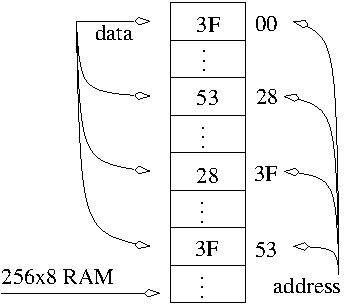
\includegraphics{Prob8-7}}
\caption{A 256x8 RAM loaded with some data.}
\label{fig:RAMhopper}
\end{figure}

\item \textbf{ (16 pts.)}
A 256x8 RAM is full of data.  Design a circuit that jumps 
around in memory.   The current address should be stored in a
register called PC.  If the MSB of the fetched word is 1, then the 
remaining seven bits represent a 7-bit 2's complement number;  add these 
seven bits to the PC.  If the MSB of the fetched word is 0 then just 
increment the PC.  Repeat this process forever.
Turn in; an algorithm the datapath and control unit, the control word 
table, the memory input equations, and output equations.  
The control unit is to be implemented using a ones hot encoding.

The desired behavior of the circuit is illustrated in 
Figure~\ref{fig:RAMhopper2}.  In this figure if PC=0 then the word at
that address (3F) has a MSB of 0 so the PC is incrementde to 1. The
word at address 1 is fetched (BC) and has an MSB of 1 so the least
significant seven bits of BC are added to the PC, making its new value
3D.  repeating this process sees the PC goto address 21, 22, 21, 22
into a never ending cycle.   Make sure the solution identifies how
to add the least significant seven bits to an 8-bit PC.

\begin{figure}[ht]
\center{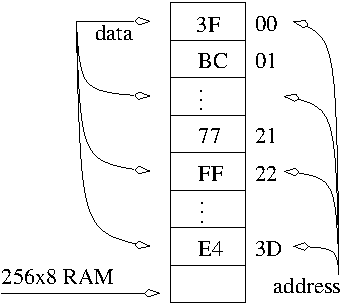
\includegraphics{Prob8-8}}
\caption{A 256x8 RAM loaded with some data.}
\label{fig:RAMhopper2}
\end{figure}

\begin{onlysolution}  \textbf{Solution} \itshape{

\begin{figure}[ht]
\center{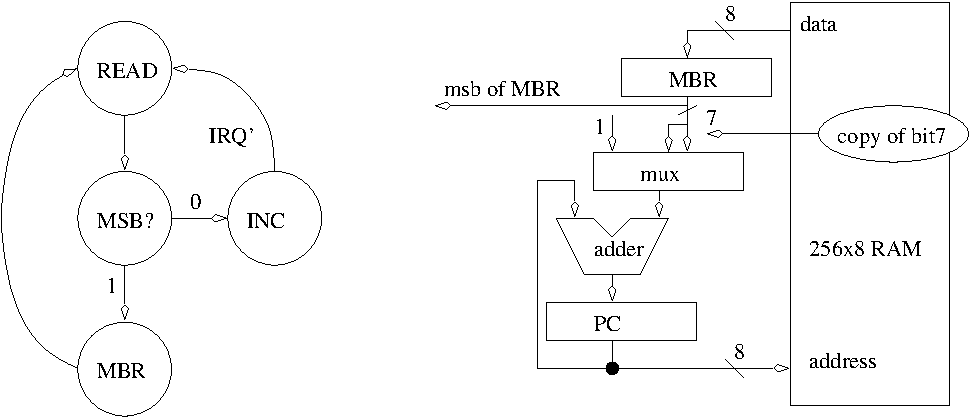
\includegraphics{Sol8-8}}
\caption{The datapath and control to conditionally hop around
in RAM.}
\end{figure}


\textbf{ Control Word}

\begin{tabular}{l|l|l|l|l|l|l}
STATE & RE     & CS     &MUX          &MBR    & PC	\\ \hline
      & 0 nada & 0 nada &0 pass 1     &0 hold &0 hold	\\ \hline
      & 1 read & 1 RAM  &1 pass MBR   &1 load &1 load	\\ \hline
      &        &        &             &       &       	\\ \hline
READ  & 1      & 1      & x           & 1     & 0	\\ \hline
MSB?  & 0      & 0      & x           & 0     & 0	\\ \hline
INC   & 0      & 0      & 0           & 0     & 1	\\ \hline
MBR   & 0      & 0      & 1           & 0     & 1	\\ \hline
\end{tabular}

\textbf{ MIEs and OEs}

\begin{tabular}{ll}
MIE					&	OE			\\
$D_{read}= Q_{mbr}+Q_{inc}$		&  $Z_{re} = Q_{read}$		\\
$D_{msb} = Q_{read}$			&  $Z_{cs} = Q_{read}$		\\
$D_{inc}= Q_{msb} m'$			&  $Z_{MUX} = Q_{mbr}$		\\
$D_{mbr}= Q_{msb} m$			&  $Z_{mbr} = Q_{read}$		\\
\end{tabular}

} \end{onlysolution} 


\item \textbf{ (16 pts.)}
Modify the circuit in the previous problem as follows.  Anytime
an external input, called IRQ, is asserted the circuit is to stop
jumping around and assert and ACK.  The outside world will then read
the PC (which must be routed outside the datapath) and then drop the 
IRQ.  The circuit should then drop the ACK and resume jumping.
Turn in; an algorithm the datapath and control unit, the control word 
table, the memory input equations, and output equations.  
The control unit is to be implemented using a ones hot encoding.


\item  \textbf{ (16 pts.)} Design a circuit that reads successive words from 
a 1kx12 RAM and
updates a 12-bit register called \textbf{ ACC} based on the upper two bits of the 
memory word.  The address of the current memory word should be contained
in a register called PC (Program Counter).  Since the words read from the
RAM will tell us what operation to perform on the ACC, the memory word will
be stored in a register called IR (Instruction Register).  If the upper
two bits of IR are:
\begin{enumerate}
\item  00 then add the lower 10 bits of the IR to ACC.  Pad the upper two
    bits of the IR with 0's before adding to the ACC.
\item  01 then store the ACC to the address specified by the 
    lower 10 bits of the IR.
\item  10 then load the ACC from from the address specified by the lower 
    10 bits of the IR.
\item  11 then clear the value of ACC to 0.
\end{enumerate}

The PC is to be initialized to 0.  After the each memory word is read
and the appropriate operation performed on ACC, the PC should be
incremented.
Turn in; an algorithm the datapath and control unit, the control word 
table, the memory input equations, and output equations.  
The control unit is to be implemented using a ones hot encoding.


\begin{onlysolution}  \textbf{Solution} \itshape{ 

\textbf{ Algorithm}
%% \begin{verbatim}
%% PC = 0;
%% while(1) {
    %% IR = RAM[PC];
    %% if (IR(11,10) == 00) 
    %% ACC += 00 & IR(9 downto 0);
    %% if (IR(11,10) == 01) 
    %% RAM[IR(9 downto 0) = ACC;
    %% if (IR(11,10) == 10) 
    %% ACC = RAM[IR(9 downto 0)];
    %% if (IR(11,10) == 11) 
    %% ACC = 0;
    %% PC += 1;
%% }
%% \end{verbatim}

\textbf{ Datapath and Control}

\begin{figure}[ht]
\center{\scalebox{0.7}{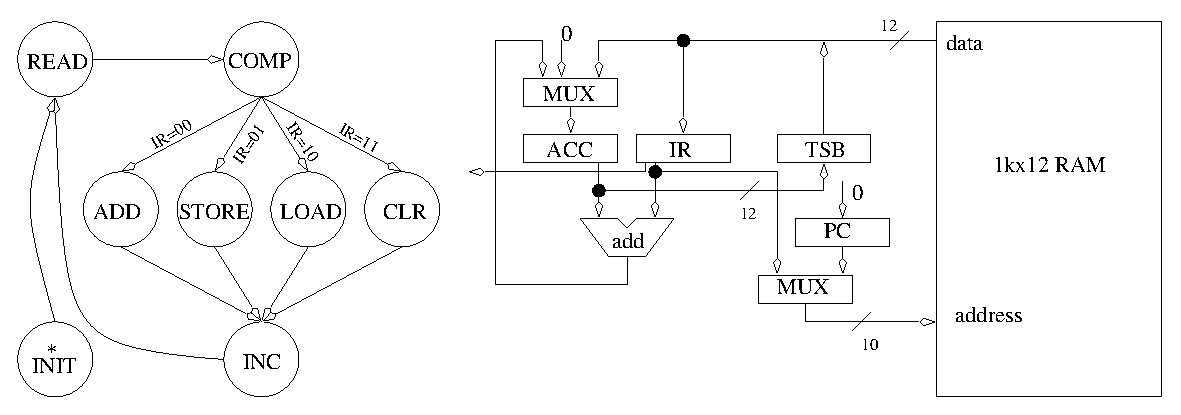
\includegraphics{Sol8-10}}}
\end{figure}

\textbf{ Control Word}

\tiny{
\begin{tabular}{l|l|l|l|l|l|l|l|l}
State & ACC mux	& Acc   & IR    & TSB   & PC	    & Addr Mux & CS	& R/W'	\\ \hline
      & 00 add & 0 hold & 0 hold & 0 Z    & 00 hold & 0 PC	& 0 no & 0 write \\ \hline
      & 01 0   & 0 load & 0 load & 1 pass & 01 load & 1 IR	& 0 on & 1 read \\ \hline
      & 10 RAM & 	& 	& 	& 10 up	&	 	& 	 & 	\\ \hline
      & 	& 	& 	& 	& 	& 	 	& 	 & 	\\ \hline
Init  &	01	& 1	& 0	& 0	& 01	&	x	& 0	& x	\\ \hline
Read  & xx	& 0	& 1	& 0	& 00	&	0	& 1	& 1	\\ \hline
Comp  & xx	& 0	& 0	& 0	& 00	&	x	& 0	& x	\\ \hline
Add   & 00	& 1	& 0	& 0	& 00	&	x	& 0	& x	\\ \hline
Stor  & xx	& 0	& 0	& 1	& 00	&	1	& 1	& 0	\\ \hline
Load  & 10	& 0	& 0	& 0	& 00	&	1	& 1	& 1	\\ \hline
Clr   & 01	& 1	& 0	& 0	& 00	&	x	& 0	& x	\\ \hline
Inc   & xx	& 0	& 0	& 0	& 10	&	x	& 0	& x	\\ 
\end{tabular}
}


\textbf{ MIEs and OEs}

\begin{tabular}{ll}
MIE                                     &       OE                      \\
$D_{Init}= Q_{wait1a}req'$            &  $Z_{m1} = Q_{load}$           \\
$D_{Read } = Q_{wait1a}req$             &  $Z_{Init} = Q_{Clr}$           \\
$D_{Comp}= Q_{getA} + Q_{wait2A}req$  &  $Z_{Acc} = Q_{Init} + Q_{Add} + Q_{Clr}$               \\
$D_{Add}= Q_{wait2a}req' + Q_{wait1B}req'$   &  $Z_{IR} = Q_{Read}$     \\
$D_{Stor} = Q_{wait1b}req$             &  $Z_{TSB} = Q_{Stor}$         \\
$D_{Load}= Q_{GetB} + Q_{wait2b}req$  &  $Z_{PC1} = Q_{Inc}$          \\
$D_{Clr  } = Q_{wait2B}req'$            &  $Z_{PC0} = Q_{Init}$          \\
$D_{Inc } = Q_{For}LB$                 &   $Z_{CS} = Q_{Read}+Q_{Stor}+Q_{Load}$     \\
                    &   $Z_{Amux} = Q_{Read}+Q_{Stor}+Q_{Load}$   \\
                    &   $Z_{RW} = Q_{Read}+Q_{Load}$            \\
\end{tabular}

}\end{onlysolution} 

\item \textbf{ (16 pts.)}
Design a circuit that moves $M$ consecutive words from address $S$ (source) to
address $D$ (destination).  For example, if $M=4$, $S=3EA$ and $D=1FE$ then the 
circuit would move words 3EA, 3EB, 3EC and 3ED to address 1FE, 1FF, 200 and 201.
Each of $M,S,D$ is preloaded into a register.  While this problem appears simple,
its really rather treacherous.  The circuit will have to handle cases where 
$S+M > D$.  In such a case the order of the data movement must be carefully planned.
In order to simplify the design, assume that $S<D$.  
Turn in; an algorithm the datapath and control unit, the control word 
table, the memory input equations, and output equations.  
The control unit is to be implemented using a ones hot encoding.
Do not worry about the sizes of the
registers or RAM.

\item \textbf{ (16 pts.)}
Design a circuit that determines how many times a user
specified 8-bit value, called \textbf{ key}, occurs in an 1kx8 RAM.  
\textbf{ key} is to be read using a two-line handshake; the circuit 
is the passive consumer.
Turn in; an algorithm the datapath and control unit, the control word 
table, the memory input equations, and output equations.  
The control unit is to be implemented using a ones hot encoding.


\item \textbf{ (16 pts.)} Design a circuit that records the number of times that it
has seen an 8-bit, user specified value, \textbf{ key}.  The key will
is shown to the circuit, at most, 16 times.  The collection of 
keys is stored in a 1kx12 RAM.  The RAM is larger
than it needs to be because it is thought that in the future
the number of keys will be increased.  Each word of the RAM is 
organized as follows; The upper eight bits hold the key and the lower
four bits hold the ``hit count", the number of times that this key has
been seen.  The circuit should read in the key using a two-line
handshake; the circuit is the passive consumer.  The circuit
should then scan the RAM looking for a matching key; a match, if
it exists, will only occur once in the RAM.  If a match is 
found then increment the lower four bit and store the key and the
incremented hit count back to RAM.  
Turn in; an algorithm the datapath and control unit, the control word 
table, the memory input equations, and output equations.  
The control unit is to be implemented using a ones hot encoding.


\item \textbf{ (36 pts.)}
Design a digital circuit to control access to an
automated parking garage containing 828 parking spaces.  
Drivers pull up to the garages gate and insert 
their pass card into a card reader.  The card reader sends the pass card
ID number to the digital circuit.  If their pass card has a valid
code then the gate opens.  There is a pressure sensor just inside the
entry way which sends a signal to the circuit whenever a significant
load is present (over 150 lbs).
The exit procedure is similar, the users have to insert their pass card
into a card reader.  The digital circuit then raises the exit gate bar,
a pressure sensor at the exit tells the circuit when it is OK to close
the exit gate.  See Figure~\ref{fig:Garage}.
\begin{figure}[ht]
\center{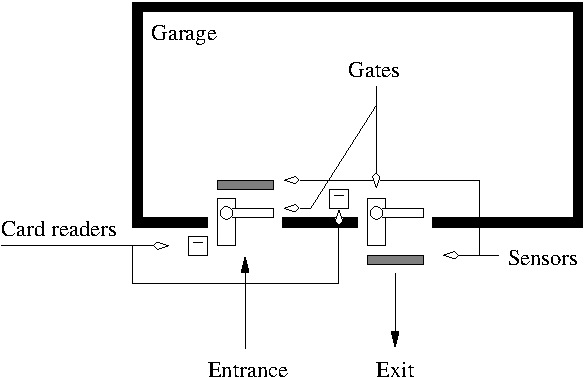
\includegraphics{Prob8-14}}
\caption{The layout of an automated garage.}
\label{fig:Garage}
\end{figure}

The signal names are defined in the following table:

\begin{tabular}{|l|l||l|l|} \hline
Entrance gate	& InGate	& 0 Close gate & 1 Open gate \\ \hline
Entrance sensor	& InSen		& 0 No weight &  1 Weight present \\ \hline
Entrance REQ	& InREQ		& 0 No card read data & 1 Card reader has data  \\ \hline
Entrance ACK	& InACK		& \multicolumn{2}{c|}{Circuit control}   \\ \hline
Entrance ID	& InID		& \multicolumn{2}{c|}{Card ID} \\ \hline
Exit gate	& OutGate	& 0 Close gate &  1 Open gate \\ \hline
Exit sensor	& OutSen	& 0 No weight & 1 Weight present\\ \hline
Exit REQ	& OutREQ	& 0 No card read data & 1 Card reader has data  \\ \hline
Exit ACK	& OutACK	& \multicolumn{2}{c|}{Circuit control}   \\ \hline
Exit ID		& OutID		& \multicolumn{2}{c|}{Card ID} \\ \hline
\end{tabular}

The gate requires a logic 1 to start and to stay open. The sensor will 
generate a logic 1 while there is more than 150 lbs. on the sensor.  Only
close the gate when the rear wheels of the car activate the
sensor (hope no unicycle use the garage).  The entrance card reader 
will provide InID or OutID using a 
two-line handshake, where the circuit is the passive consumer.
Assume that at any point in time only one car is
entering or leaving the garage.  That is, deal with only
one direction at a time.

In addition to controlling access to the garage, the clients would also
like to keep track track of how many times a pass ID has been used to
gain access in-to and out-of the garage.  The count will be checked and
reset once a month.  Cars pass into and out of the garage at most 4
times a day.

To implement this circuit use a \textit{ single} RAM.  Each word of the
RAM must be divided into three fields; ID, Ins and Outs corresponding to
the pass ID number, number of times into the garage and number of times
out of the garage respectively.   The digital circuit will scan successive
IDs in the RAM looking for a match.  If a match 
is found then either increment the Ins or Outs field then store this 
item back into the RAM.  A major issue in this design is determining
the sizes of the data items.  Use the information in the word statement
to make the design as space efficient as possible.
\begin{figure}[ht]
\center{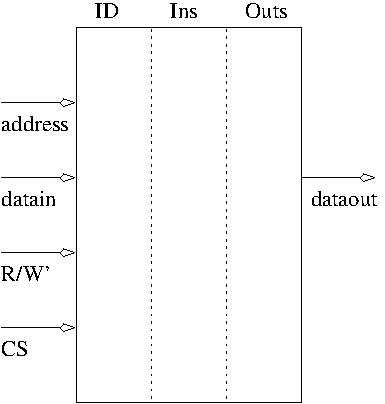
\includegraphics{Prob8-14b}}
\caption{The format of the RAM in the garage circuit problem.}
\label{fig:GarRAM}
\end{figure}
Turn in; an algorithm the datapath and control unit, the control word 
table, the memory input equations, and output equations.  
The control unit is to be implemented using a ones hot encoding.


\item \textbf{ (16 pts.)} Design a circuit that converts a 6-bit binary number into a 2 
digit BCD representation.  The circuit acquires a 6-bit number through
a two-line handshake where the circuit is a passive consumer.  The 
circuit is then to convert this 6-bit number into two BCD digits and
signals it completion via a DONE signal.

A number X can be converted from binary into BCD digits by iteratively
checking that X is greater than 10, then subtracting 10 from X.  Each
subtraction should increment a tens digit counter.

Make sure to identify the size of all the signals in the datapath
and the size of any register, counters, etc...
Turn in; an algorithm the datapath and control unit, the control word 
table, the memory input equations, and output equations.  
The control unit is to be implemented using a ones hot encoding.

 
\item \textbf{ (8 pts.)}
Design a circuit that converts a 2 digit BCD number into a
binary number.  The circuit acquires the BCD digits through 2 read
operations most significant digit first.  Each read operation takes 
the form of a two-line handshake where the circuit is a passive 
consumer.

A 2 digit BCD number can be converted into binary by multiplying the
most significant digit by 10 then adding it to the least significant
BCD digit.  A number can be multiplied by 10 using the shift-and-add
technique presented on page~\pageref{page:MulyBy10}.  Note, this
task can be accomplished without using a single shift register.
For example, the adder in Figure~\ref{fig:NineTimes} generates the value
of 9*X from a 4-bit register by adding X, shifted left by three bits, to X.

\begin{figure}[ht]
\center{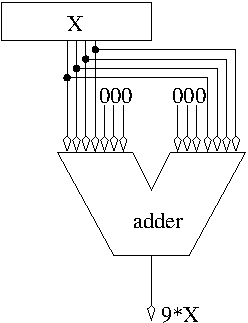
\includegraphics{Prob8-16}}
\caption{A simple circuit to compute 9*X.}
\label{fig:NineTimes}
\end{figure}

Make sure to identify the size of all the signals in the datapath
and the size of any register, counters, etc...
Turn in; an algorithm the datapath and control unit, the control word 
table, the memory input equations, and output equations.  
The control unit is to be implemented using a ones hot encoding.

 
\item \textbf{ (36 pts.)}
Design a digital circuit that plays a game of
roulette, allows betting and keeps track of total earnings.
The roulette wheel has 8 slots, labeled $1 \ldots 8$.  The player
can play one of the numbers straight or play even or odd.
The player starts with \$10. 
The layout of the machine is shown in Figure~\ref{fig:Roulette}.
\begin{figure}[ht]
\center{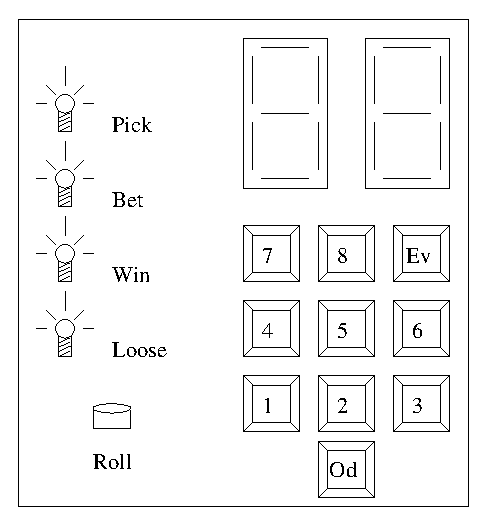
\includegraphics{Prob8-17}}
\caption{The layout of the roulette playing machine.  
The two 7-segment displays at the top are used for a variety
of purposes.}
\label{fig:Roulette}
\end{figure}

The sequence of events is as follows:
\begin{enumerate}
\item	The circuit lights up the PICK LED.
    The player enters their guess; a number between 1-8, even or odd.
    While holding down their guess they press the roll button.
\item	The circuit displays the picked number in the left most
    7-segment display.  The circuit lights up the BET LED.
    The player enters a one digit bet between 1 to 8.  While holding
    down their bet they press the roll button.
\item 	The circuit displays the bet on the rightmost 7-segment
    display.
    The player pushes and holds down the roll button.
    The circuit increments a mod 8 counter while the roll 
    button is depressed. It would be nice to display the
    current count value on right 7-seven segment display.
    Since the clock cycle is on the order of milliseconds,
    then the user would not be able to anticipate the roll.
\item	The player releases the roll button.  The final roll
    is displayed on the rightmost 7-segment display.
    The circuit stops incrementing the counter and checks
    to see if the final value matches the players guess.
    If the match is correct then light the WIN LED and
    increment the players earnings.  If the match is incorrect
    then light the LOOSE LED and decrement the players
    earnings.
\item	The play hits the roll button to clear the roll information
    from the 7-segment displays.
\item	The circuit displays the players earnings on the 7-segment
    display.
\item	When the user pushes the roll button then go to step 1.
\end{enumerate}

Set reasonable bounds on the maximum winnings.  Values may be displayed
in hexadecimal (assume there is a hex to 7-segment display converter
available).  See page~\pageref{page:7seg} for more
information.
Turn in; an algorithm the datapath and control unit, the control word 
table, the memory input equations, and output equations.  
The control unit is to be implemented using a ones hot encoding.


\begin{onlysolution}  \textbf{Solution} \itshape{

\textbf{ Algorithm}

%% cash = 10; 
%% left_seven = blank; 
%% right_seven = cash; 
%% while(cash > 0) { 
%%     led_array = 1 0 0 0;    // Pick Bet Win Loose 
%%     while(ROLL == 0); 
%%     guess = Datain; 
%%     while(ROLL == 1); 
%%      
%%     led_array = 0 1 0 0;    // Pick Bet Win Loose 
%%     left_seven = guess; 
%%     right_seven = blank; 
%%     while(ROLL == 0); 
%%     bet = Datain; 
%%     while(ROLL == 1); 
%%      
%%     led_array = 0 0 0 0;    // Pick Bet Win Loose 
%%     right_seven = bet; 
%%     while(ROLL == 0); 
%%     while(ROLL == 1) count = count + 1; 
%%  
%%     right_seven = count; 
%%     if (count == guess) { 
%%         cash = cash + (bet << 2); 
%%         led_array = 0 0 1 0;    // Pick Bet Win Loose 
%%     } else { 
%%         cash = cash - bet; 
%%         led_array = 0 0 0 1;    // Pick Bet Win Loose 
%%     } 
%%     while(ROLL == 0); 
%%     while(ROLL == 1); 
%%     right_seven = cash; 
%%  
%% }	 
%% led_array = 0 0 0 1;    // The user is out of money 
%% while(1);		// Halt the machine 
 
\textbf{ Datapath and Control}

\begin{figure}[ht]
\center{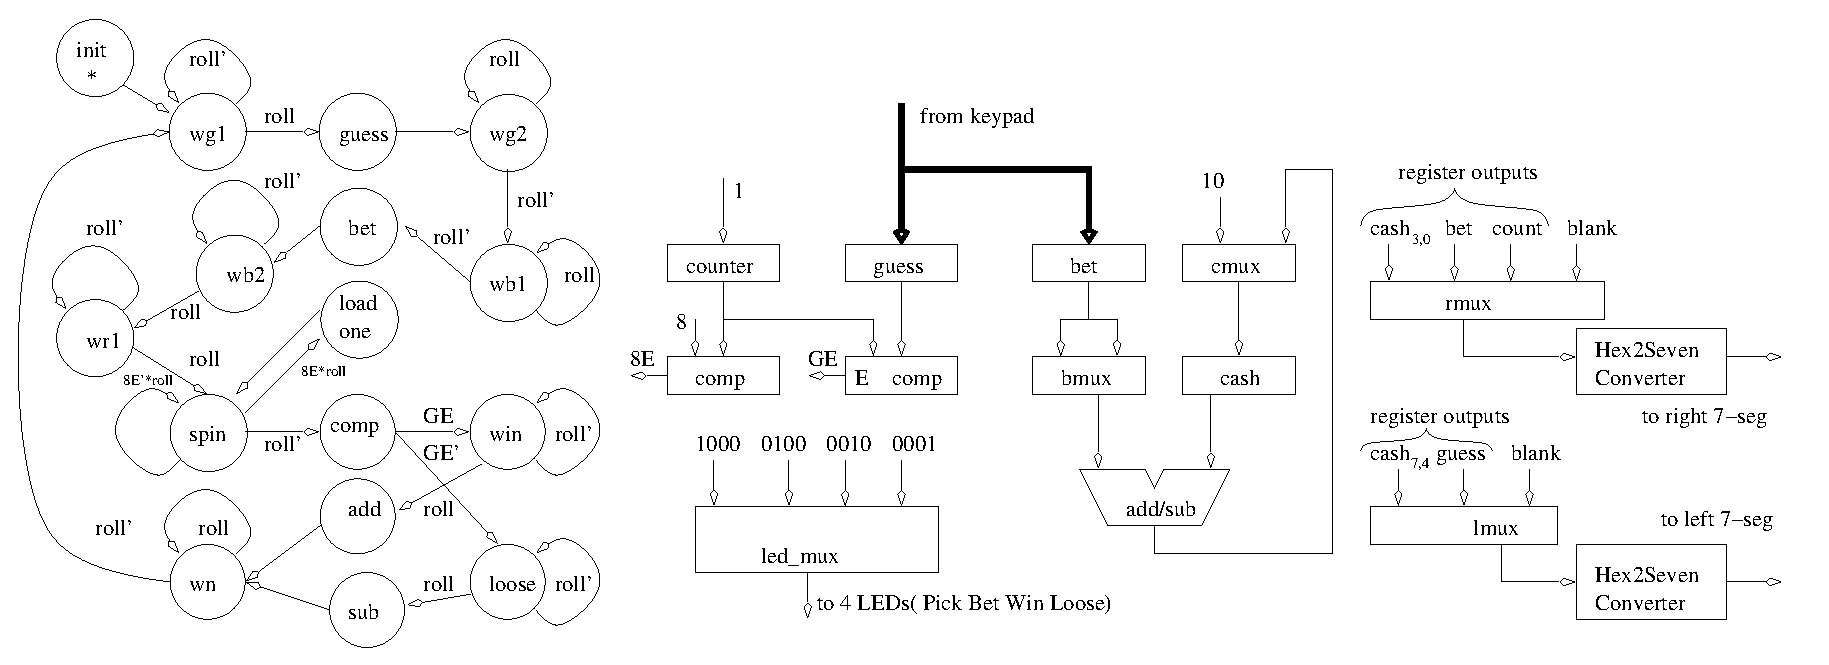
\includegraphics{Sol8-16}}
\end{figure}

Note from the figure that, the user may acquire
up to 0xFF cash.  Each hex digit of the users total cash will 
be displayed on its own 7-segment display.

\textbf{ Control Word}

{\tiny
\begin{tabular}{l|l|l|l|l|l|l|l|l|l|l}
State &  counter& guess  & bet    & cmux      & bmux     & cash   & add/sub & ledmux    & rmux   & lmux \\ \hline
      & 00 hold & 0 hold & 0 hold & 0 \$10    & 0 bet    & 0 hold & 0 add  & 00 (pick) &00 cash &00 cash  \\ \hline
      & 01 load & 0 load & 1 load & 1 add/sub & 1 bet<<2 & 1 load & 1 sub  & 01 (bet ) &01 bet  &01 guess \\ \hline
      & 10 up   &        &        &  	      &          &        &        & 10 (win ) &10 count&10 blank \\ \hline
      &         &        &        &  	      &          &        &        & 11 (loose)&11 blank&         \\ \hline
      &         &        &        &  	      &          &        &        &          &         &   \\ \hline
init  & 00      & 0      &  1     & 0	      & x        &  1     &  x     & 00       &  11     & 11\\ \hline
wg1   & 00      & 0      &  0     & x	      & x        &  0     &  x     & 00       &  00     & 00\\ \hline
guess & 00      & 1      &  0     & x	      & x        &  0     &  x     & 00       &  11     & 01\\ \hline
wg2   & 00      & 0      &  0     & x	      & x        &  0     &  x     & 00       &  11     & 01\\ \hline
wb1   & 00      & 0      &  0     & x	      & x        &  0     &  x     & 01       &  11     & 01\\ \hline
bet   & 01      & 0      &  1     & x	      & x        &  0     &  x     & 01       &  11     & 01\\ \hline
wb2   & 00      & 0      &  0     & x	      & x        &  0     &  x     & 00       &  01     & 01\\ \hline
wr1   &         &        &        & x	      & x        &        &  x     &          &         &   \\ \hline
spin  & 10      & 0      &  0     & x	      & x        &  0     &  x     & 00       &  10     & 01\\ \hline
load 1& 01      & 0      &  0     & x	      & x        &  0     &  x     & 00       &  10     & 01\\ \hline
comp  & 00      & 0      &  0     & x	      & x        &  0     &  x     & 00       &  10     & 01\\ \hline
win   & 00      & 0      &  0     & 1	      & 1        &  1     &  0     & 10       &  10     & 01\\ \hline
add    &         &        &        &  	      &          &        &        &          &         &   \\ \hline
loose & 00      & 0      &  0     & 1	      & 0        &  1     &  1     & 11       &  10     & 01\\ \hline
sub   &         &        &        &  	      &          &        &        &          &         &   \\ \hline
wn    & 00      & 0      &  0     & x	      & x        &  0     &  x     & 00       &  00     & 00\\ 
\end{tabular}
}

\textbf{ MIEs and OEs}

$$
\begin{array}{ll}
MIE						&       OE                      \\
D_{init}= 0					&  Q_{c1} = Q_{spin}          \\
D_{wg1}= Q_{wg1}*roll'+Q_{wn}*roll'		&  Z_{c0} = Q_{bet} + Q_{load1}           \\
D_{guess} = Q_{wg1}*roll           		&  Z_{guess} = Q_{guess}           \\
D_{wg2}= Q_{guess} + Q_{wg2}*roll		&  Z_{bet}= Q_{init} + Q_{bet} \\
D_{wb1}= Q_{wg2}*roll'+Q_{wb1}*roll		&  Z_{cmux} = Q_{win}+Q_{loose}           \\
D_{bet } = Q_{wb1}*roll'			&  Z_{bmux} = Q_{win}           \\
D_{wb2}= Q_{bet} + Q_{wb2}*roll'		&  Z_{cash} = Q_{init} + Q_{win} + Q_{loose}    \\
D_{spin}= Q_{wb2}roll + Q_{spin}*8E'roll + Q_{load1}  &  Z_{addsub} = Q_{loose}     \\
D_{load1}= Q_{spin}*8E*roll    		& Z_{led1} = Q_{win} + Q_{loose} \\
D_{comp} = Q_{spin}roll'			& Z_{led0} = Q_{wb1}+Q_{bet}+Q{loose}         \\
D_{win}= Q_{comp}*GE				& Z_{rseg1} = not (Q_{wg1}+Q_{wb2}+Q_{wn})      \\
D_{loose} = Q_{comp}*GE'			& Z_{rseg0} = Q_{init,guess,wg2,wb1,bet,wb2}\\
D_{wn2} = Q_{wn}*roll + Q_{win}*roll + Q_{loose}*roll & Z_{lseg1} = Q_{init}  \\
\end{array} $$

} \end{onlysolution} 

\item \textbf{ (20 pts.)}
Design a tone generator.  The tone generator is a box with two buttons
on it labeled ``Up" and ``Down" and a 1-bit output.  At start-up the tone 
generator outputs
a 440Hz square wave (clock-like signal).  Every time that the Up button
is pressed the tone generator should increase the frequency of the square
wave by $\sqrt[12]{2}-1.0 = 0.059463094 \approx 7/128$ of its current frequency.  
To determine the fraction $7/128$ of $X$, shift $X$ left by 7-bits (dividing by
128) then multiplying it by 4+2+1.  Every time that the down button is pressed
the circuit should decrease the frequency by 7/128 of its current value.  Assume
that the master clock frequency of the circuit is 4Mhz.  Turn in 
any relevant calculations, algorithm, datapath and control, control word,
MIEs, OEs and the maximum tone frequency of the circuit.
Turn in; an algorithm the datapath and control unit, the control word 
table, the memory input equations, and output equations.  
The control unit is to be implemented using a ones hot encoding.


\end{enumerate}

